\documentclass[11pt,a4paper]{book}

\usepackage{mypackage} % moje definice a styly


\faculty{Faculty of science}
\department{Department of theoretical physics and astrophysics}
\university{Masaryk University}
\thesisType{Ph.D. Dissertation}
\city{Brno}
\academicYear{2022/2023}
\yearOfMaking{2022}
\thesisTitle{Analysis and Modelling of Non-linear \newline Dynamical Systems in Astrophysics}
\thesisTitleEN{Analysis and Modeling of Non-linear \newline Dynamical Systems in Astrophysics}
\thesisTitleCZ{Analýza a modelování nelineárních dynamických systémů v astrofyzice}
\author{Jiří Květoň}
\authorFull{Mgr. Jiří Květoň}
\supervisor{Mgr. Filip Hroch Ph.D.}
\consultant{Mgr. Viktor Votruba Ph.D.}
\coverImage{./img/cover.png}

% References package defs
\usepackage[backend=biber,natbib, style=authoryear, citestyle=authoryear, maxcitenames=2, sorting=ynt]{biblatex}

% References file
% pozn. https://tex.stackexchange.com/questions/305381/biblatex-empty-bibliography ... kvuli chybe nedefinovanych bib
\addbibresource{./references.bib}

\usepackage[binary-units]{siunitx}

\usepackage{tikz}
\usetikzlibrary{shapes.geometric, shapes.misc, arrows}

\tikzstyle{startstop} = [ellipse, minimum width=5.5cm, minimum height=1 cm, inner sep=0.2cm, text centered, draw=black, fill=red!25]
\tikzstyle{process} = [rectangle, minimum width=5.5cm, minimum height=1 cm, inner sep=0.2cm, text centered, text width=5.5cm, draw=black, fill=blue!25]
\tikzstyle{decision} = [chamfered rectangle, minimum width=5.5cm, minimum height=1 cm, inner sep=0.25cm, text centered, text width=5.5cm, draw=black, fill=green!25]
\tikzstyle{arrow} = [thick, ->, >=latex]

\usepackage{rotating}

\usepackage{enumitem}
\usepackage{varwidth}
% \setlist[itemize]{leftmargin=30mm,itemsep=0mm}

\def\CC{{C\nolinebreak[4]\hspace{-.05em}\raisebox{.4ex}{\tiny\bf ++}}}

\begin{document}
    % Pro uvodni strany se vypne cislovani
    \pagenumbering{gobble}

    % --
    % Titulní strana prace
    % --
    \maketitle
    \blankpage

    % --
    % Originální zadání
    % --
    % scale a offset aby marginy vicemene sedely do rozmeru ostatnich stranek
    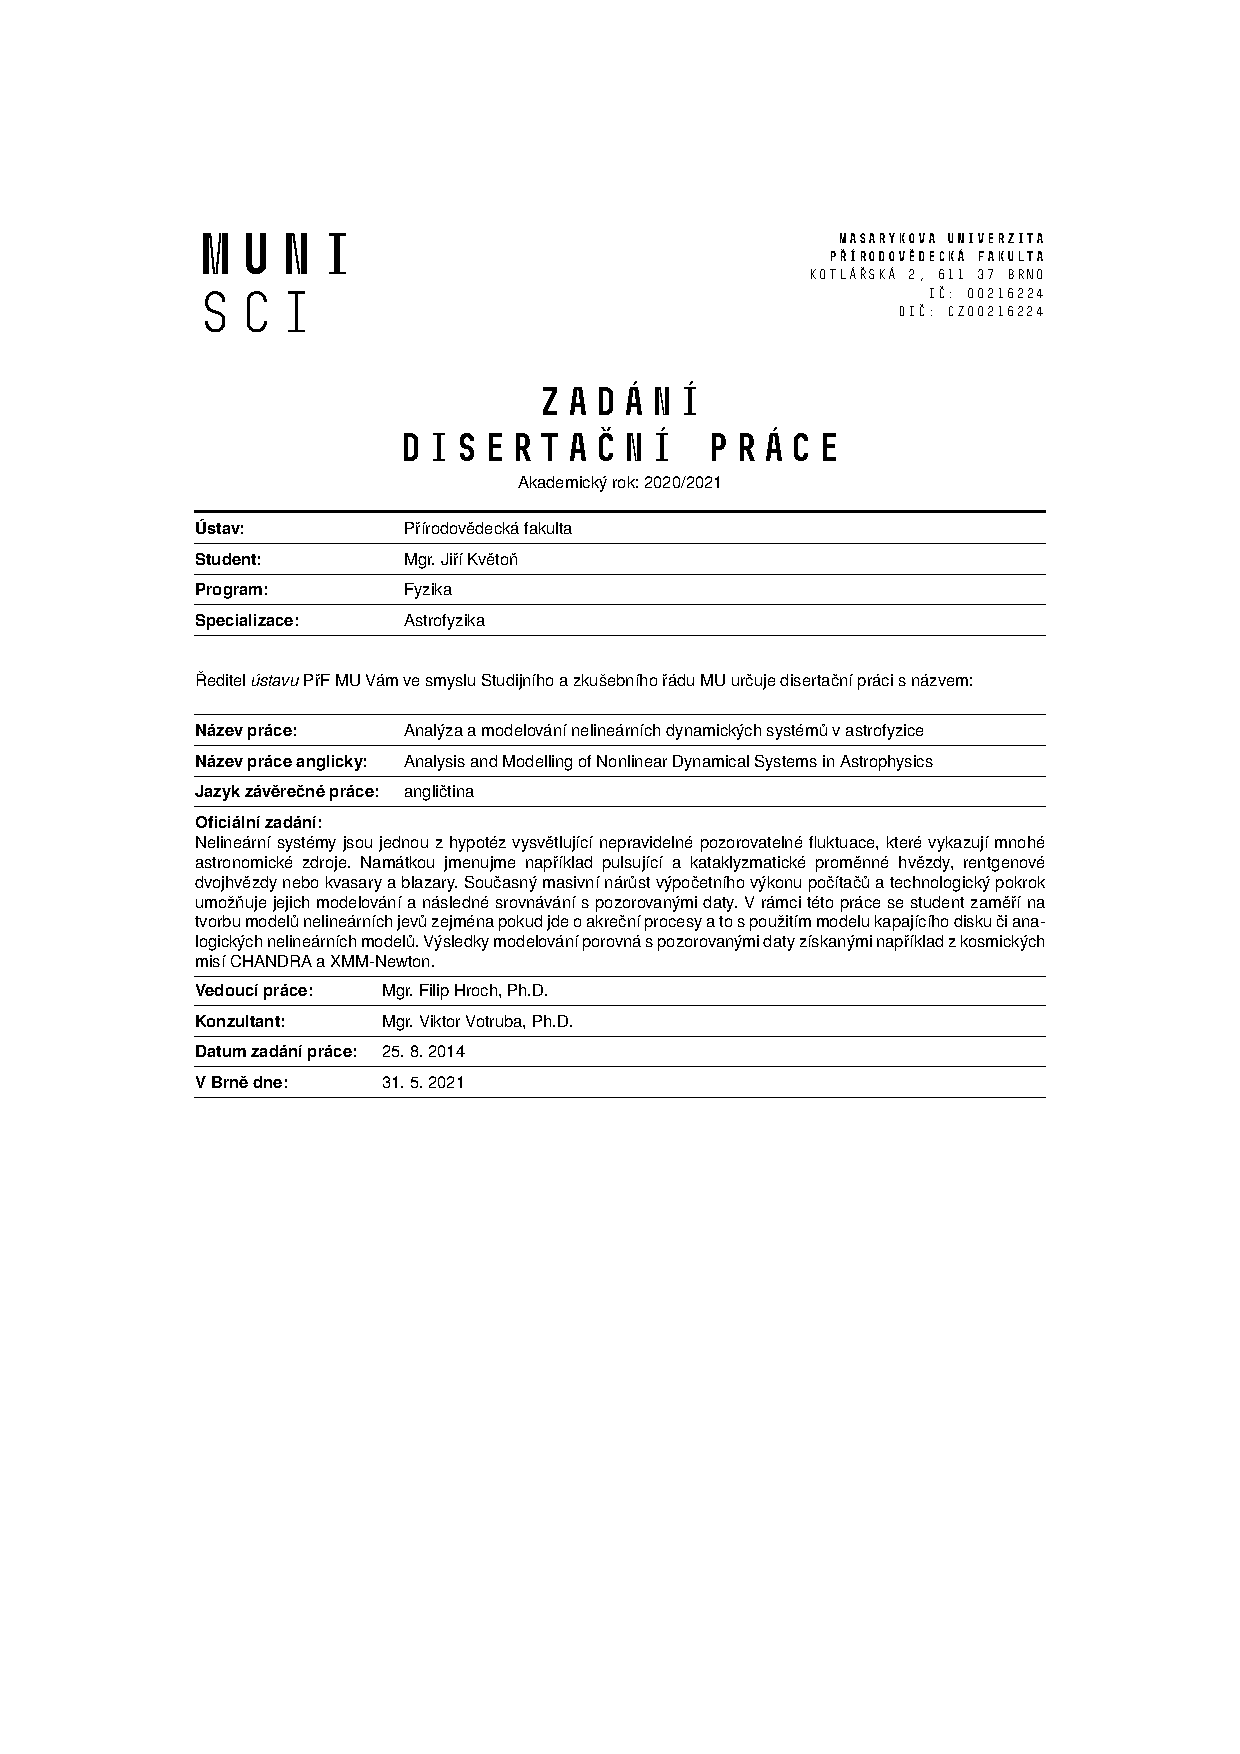
\includepdf[scale=0.85]{./misc/zadani.pdf}
    \blankpage

    \pagestyle{plain}

    % --
    % Bibliografický záznam
    % --
    %\phantomsection
    \bibinfoen

    %\phantomsection
    \bibinfocz

    % --
    % Abstrakt (CZ+EN)
    % --
    %\phantomsection
    \shortchapter{abstract}{./misc/abstract-en.tex}
    \blankpage

    %\phantomsection
    \shortchapter{abstrakt}{./misc/abstract-cz.tex}
    \blankpage

    % --
    % Poděkování
    % --
    %\phantomsection
    \shortchapter{acknowledgments}{./misc/acknowledgments.tex}
    \blankpage

    % --
    % Prohlášení
    % --
    %\phantomsection
    \declaration{./misc/declaration.tex}
    \blankpage

    % --
    % Copyright
    % --
    \copypage
    \blankpage

    % --
    % Obsah
    % --
    \content

    % Zapnout cislovani a vlastni styl hlavniho textu
    \pagestyle{mystyle}
    \pagenumbering{arabic}
    \setcounter{page}{1}    

    % 1. INTRODUCTION
    \chapter{INTRODUCTION}
\thispagestyle{empty}

\mquote{The Universe is under no obligation to make sense to you.}{Neil deGrasse Tyson}




    % 2. ACCRETION DISCS
    \chapter{ACCRETION DISKS}
    \label{chap:accretion_disks}
    The term \emph{accretion} comes from a Latin word \emph{accrescere} which literarily means \emph{become larger}, and in astrophysics, we refer exactly to that process. That is the \emph{coming together and cohesion of matter under the influence of gravity to form larger bodies} (citace). One could easily argue that it is one of the most fundamental processes in the universe. From the giant galaxies to the tiniest rocks floating around in the solar system. All the stars, planets, and all there is were smashed together by gravity at some point in the past. Atom by atom, piece by piece, to form larger and larger structures. Even the dinosaurs probably met their fate by a city-sized asteroid that accreted Earth some 65 million years ago. 

\section{Accreting systems}
    Accretion is not only the mass moving and colliding but also energy taking different forms in the process. Depending on the nature of the accreting system and its central object, radiation of various types is emitted by the accreted matter as it loses energy. Under certain conditions, the matter flow forms an accretion disk often closely confined to the orbital plane. If we sort accreting astrophysical systems based on their size, radiation power, and a few other characteristics, we can devise a crude classification of them. We will briefly describe the accreting system types in the following sections. 

\subsection{Active galactic nuclei (AGN) and Quasar}
    The high-luminosity region containing a supermassive black hole in most galaxies' centers is refered to as \emph{Active Galactic Nucleus}. The radiative power of the AGN is usually higher than that of the whole host galaxy, and the radiation characteristics indicate that stars are not the primary source of this radiation. Instead, mass accretion onto the central supermassive black hole is the more likely source of this excess non-stellar power output. 

    The main distinguishing characteristic of AGNs is whether they are \emph{radio loud} or \emph{radio quiet}, which depends on the existence of jets that are the source of radio radiation. By \emph{jets}, we mean relatively narrow streams of accreted mass ejected from the black hole in both directions, roughly colinear with its axis of rotation. These mass ejections can travel at relativistic speeds and reach thousands of light-years away from the source object. 

    Figure \ref{fig:centaurus_a_multiwave} shows the Centaurus A (NGC 5128) galaxy with a supermassive black hole in its center. This object is a typical \emph{radio loud} AGN. We can see both jets in the radio part of the spectrum and the accreted matter in other parts of the spectrum. For example, the galaxy,s dust core is most apparent in visible light.

    A particular sub-category of AGN is Quasars. The name \emph{Quasar} is a contraction of the phrase \emph{quasi-stellar radio source} because, in the 1950s, they were detected as radio sources of unknown physical characteristics and also in visible light as faint \emph{star-like} sources. However, they are nothing like stars. These highly luminous objects are observed to the highest values of redshift. The current record holder for the most distant Quasar is the J0313-1806 detected at redshift $z = 7.64$ by \cite{wang2021}. 

    Due to the extreme distance, it is impossible, at least with today's methods, to distinguish the active core (i.e., the supermassive black hole), whose mass can range from $10^6 M_{\odot}$ to $10^{9} M_{\odot}$. To this day, more than a million quasars have been discovered, with the closest known Markarian 231 (UGC 8058) at 581 million light-years away \cite{gaia2018}. 

    \begin{figure}
        \centering
        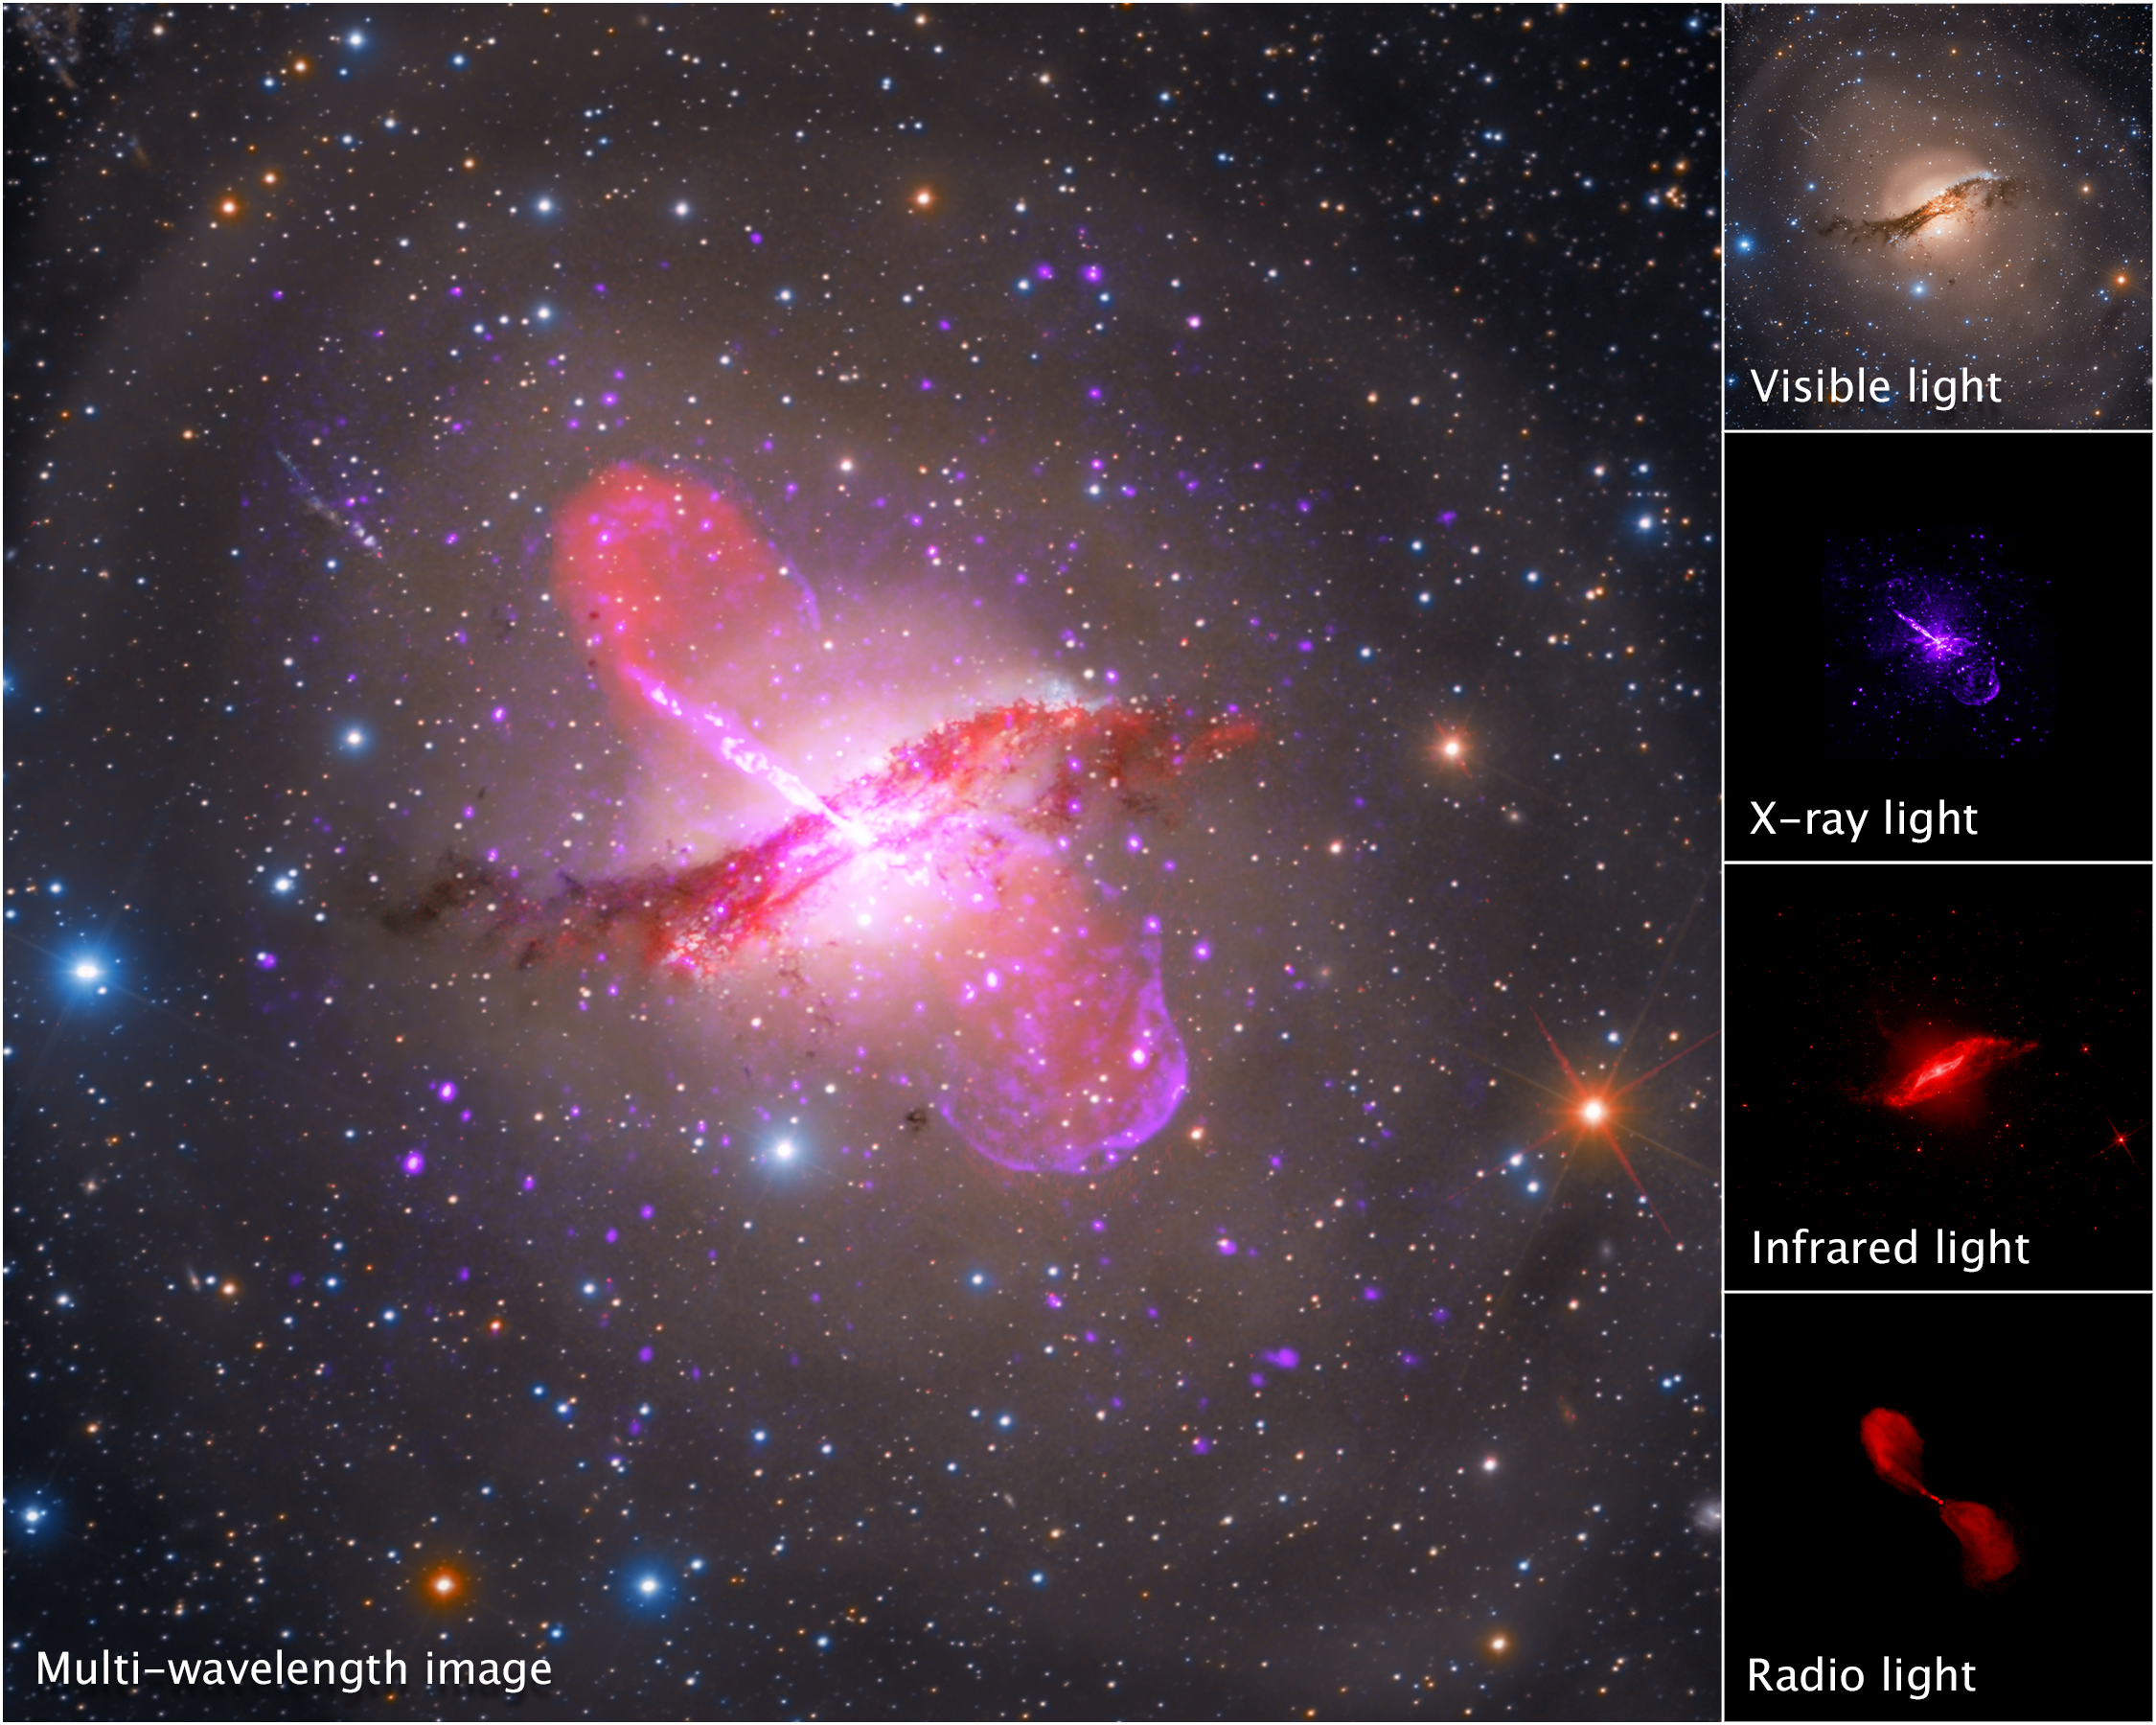
\includegraphics[width=\columnwidth]{img/multiwave_centaurus_a_agn.png}
        \caption{Multi-wavelength composition (left) and multiple narrow wavelength observations (right) of Centaurus A. Taken from \cite{nasa_img_centaurus_a}}
        \label{fig:centaurus_a_multiwave}
    \end{figure}

\subsection{X-ray binaries (XB)}
    The main sequence star in orbit around a neutron star (NSB - \emph{Neutron Star Binary}) or a black hole (BHB - \emph{Black Hole Binary}) is referred to as a \emph{X-ray binary} (XRB). The gravitational potential of these systems is strong enough that the accreted matter produces energy output up to the X-rays. Based on the mass of the primary component (i.e., the accretor), this class of binary stars is also usually split between \emph{Low-mass X-ray binary} (LXRB) and \emph{High-mass X-ray binary} (HXRB). 

    Most XRB objects go through periods of high activity when they emit twin jets at relativistic speed, not that dissimilar to AGN but at a smaller scale, and then a period of relative quiescence.

    In the special case, when the accretor is the strongly magnetized young neutron star, the accretion disk is truncated by its magnetic field or not present at all, and the matter transfers onto the neutron star by \emph{column accretion}.

    %% TODO: Muj Cygnus X-1 pro demonstraci

\subsection{Young stellar objects (YSO)}
    When a proto-star is formed from a collapsing molecular cloud, the gas and solid particles envelope forms a rotating protoplanetary accretion disk. Instabilities and self-gravity in the disk's body eventually lead to planets and other smaller objects forming. The proto-star is only detectable in infrared due to the relatively dense surrounding matter that obscures it. 

    The YSO classification consists of five classes (0-IV) based on the infrared and visible spectral energy distribution. Class 0 is a collapsing molecular cloud. Classes I to III are YSO with a formed proto-planetary disk in various stages of evolution, and lastly, class IV refers to a fully formed zero-aged star. 

    \begin{figure}[h]
        \centering
        \includegraphics[width=\columnwidth]{img/jwst_protostar_l1527.png}
        \caption{Proto-star L1527 captured by Near-Infrared-Camera (NIRCam) onboard the JWST. Taken from \cite{nasa_img_l1527}}
        \label{fig:jwst_protostar_l1527}
    \end{figure}


    As a side note, the \emph{James Webb Space Telescope} (JWST) was released only a year ago, on December 25, 2021. It is equipped with multiple near-infrared and infrared instruments, so it is literarily able to see through the clouds of such objects and uncover the stars being born. Due to JWST's observational capabilities and the sheer size of its primary mirror, we have something to look for in this particular field of astrophysical research. The first glimpses of JWST observations demonstrate the spectacular Figure \ref{fig:jwst_protostar_l1527}, showing the proto-star L1527 captured by the Near-Infrared-Camera (NIRCam). 

\subsection{Gamma-ray bursts (GRB)}
    Highly energetic, collimated flashes of $\gamma$-rays that can last tens of milliseconds up to several hours are called \emph{Gamme-ray burts} (GRB). These are considered the most energetic events in the observable universe. In addition, GRBs are accompanied by simultaneous radiation on longer wavelengths (e.g., X-ray) and a follow-up slowly fading afterglow that may be observable for up to several years. 

    It is theorized that the possible origin of GRBs may be a compact object merger or a \emph{collapsar} (i.e., the failed supernovae). The observations indicate the formation of a black hole with an accretion disk surrounding it and a high mass accretion rate \cite{piran2005}.

    One of the brightest detected GRB 221009A (Swift J1913.1+1946) was detected very recently on October 9, 2022, by the orbital \emph{Neil Gehrels Swift Observatory} \cite{grb_221009a}. It is also one of the closest observed GRBs. 

    %% TODO: obrazek GRBu??? -> spis neni potreba

\subsection{Cataclysmic variables (CV)}
    We are particularly interested in CVs in this study because our modeling efforts in the latter chapters focus on generic CV systems. Unlike the LMXB or HMXB, where the primary component is either a black hole or neutron star, the accretor in CV is a White Dwarf (WD), and its companion is a late-type star. Due to its nature, this system has a relatively weaker gravitational potential; therefore, its radiation energy output is lower than that of the XRB and is comparable in size to planetary or Earth-Moon-like systems. 

    The primary WD is a stellar core remnant composed of very dense electron-degenerate gas, and its size can be approximated by the \emph{mass-radius ratio} \cite{shapiro1983}

    \begin{equation}
        r_{\textrm{in}} \sim M^{-1/3}_{\textrm{p}},
        \label{eq:mass_radius_ratio}
    \end{equation}

    where $M^{-1/3}_{\textrm{p}}$ represents the WD mass and $r_{in}$ its radius, which also corresponds to the inner boundary layer radius of the accretion disk.

    The secondary component star fills its Roche lobe, and the overflowing matter falls onto the WD through the Langrangian point $L_1$ \cite{warner1995}. If the WD is not magnetized or weakly magnetized, the gas stream forms an accretion disk around the WD that eventually reaches its surface. In the case of strongly magnetized WD, the accretion disk is truncated or non-existent, and the magnetic field lines direct the accretion flow (citace). 

    Another important parameter of the CV binary system is its component separation distance, closely related to individual component masses. It determines the accretion disk size because the gravitational potential constrains its outer edge. The outer disk radius is calculated

    %% TODO: Citace vypoctu? Podrobnejsi vyjadreni

    \begin{equation}
        r_{out} = d \left[ \frac{M_{\textrm{s}}}{3(M_{\textrm{p}}+M_{\textrm{s}})} \right]^{1/3},
        \label{eq:disk_outher_radius}
    \end{equation}

    where $M_{\textrm{s}}$ represents the secondary component's mass and $d$ is the distance between the components. Equations \eqref{eq:mass_radius_ratio} and \eqref{eq:disk_outher_radius} give us the inner and outer constraints to define the geometry of the model, which we will define in the latter chapters of this study.   

\section{Accretion disks models}
    For the accreting matter that dissipates energy and is not supported by internal pressure, the matter will form an accretion disk, which is its minimal energy configuration. The falling matter must lose angular momentum to reach the central object. This process is done through a \emph{viscous disipation} that is key in transporting the angular momentum outward and heats the disk. The nature and magnitude of the viscous processes are the questions of accretion disk modeling because they are the critical factor determining the disk size, shape, optical dept, and radiation properties. It still needs to be better understood in the case of accretion disk matter flow because the disk's body consists of a sheering, radiative, and supersonic medium with a high Reynold's number \cite{pringle1981}, and that is quite a challenging problem to model. 

    Then there is a question of magnetic fields. The central object (i.e., WD or NS) may or may not be magnetized. Some objects rotate very fast. For example, NS rotation periods range from a couple of milliseconds to tens of seconds. The temperature and composition of the material inflow can widely differ depending on the characteristics of the secondary object. All those factors add up and create a complex non-linear accretion environment. Therefore, when modeling such a complex and dynamic astrophysical system, we are inevitably forced to make some simplifications, neglections, and approximations. 

    In many cases, the accretion disk is closely confined to an orbital plane, so in the first approximation, we may regard the disk's matter flow as two-dimensional, ad we call this the \emph{thin disc approximation}. This simple yet very effective simplification enables the creation of a very elaborate accretion model's theory, but with reduced complexity, \cite{acpow}.

\subsection{Sub-Eddington accretion disks}
    The standard vertically \emph{thin} accretion disk is formed under the conditions of sub-Eddington accretion rate and very high opacity. The Eddington limit is the maximum luminosity of a radiating body in hydrostatic equilibrium, which means the radiation and gravitational forces acting in opposite directions are in balance. The accreting matter follows very tight spiraling orbits that are almost Keplerian. Moreover, thin disks have a relatively high luminosity with spectral energy distribution closely resembling a \emph{black body} radiation. Thin disks theory was devised almost independently by \cite{lyndenbell1974}, \cite{pringle1981}. Under the umbrella of \emph{standard thin disks} is also the Shakura-Sunyaev $\alpha$-disc model, which is described more closely in Section \ref{sec:alpha_model_definition}. This model is particularly interesting to us because part of our simulation efforts in the latter chapters is focused on the $\alpha$ parameter modeling.

    In the case of the central object in the thin disc system being a black hole, the models need to deal with relativistic effects in its proximity. Researchers D. N. Page and K. S. Thorne provided such a theory in \cite{page1974}, which was later used by \cite{luminet1979} and \cite{marck1996} to generate synthetic images of Keplerian disk around a black hole distorted by intense gravitational lensing. Figure \ref{fig:bh_warped} shows a more recent simulation example of such a synthetic image. 

    \begin{figure}[h]
        \centering
        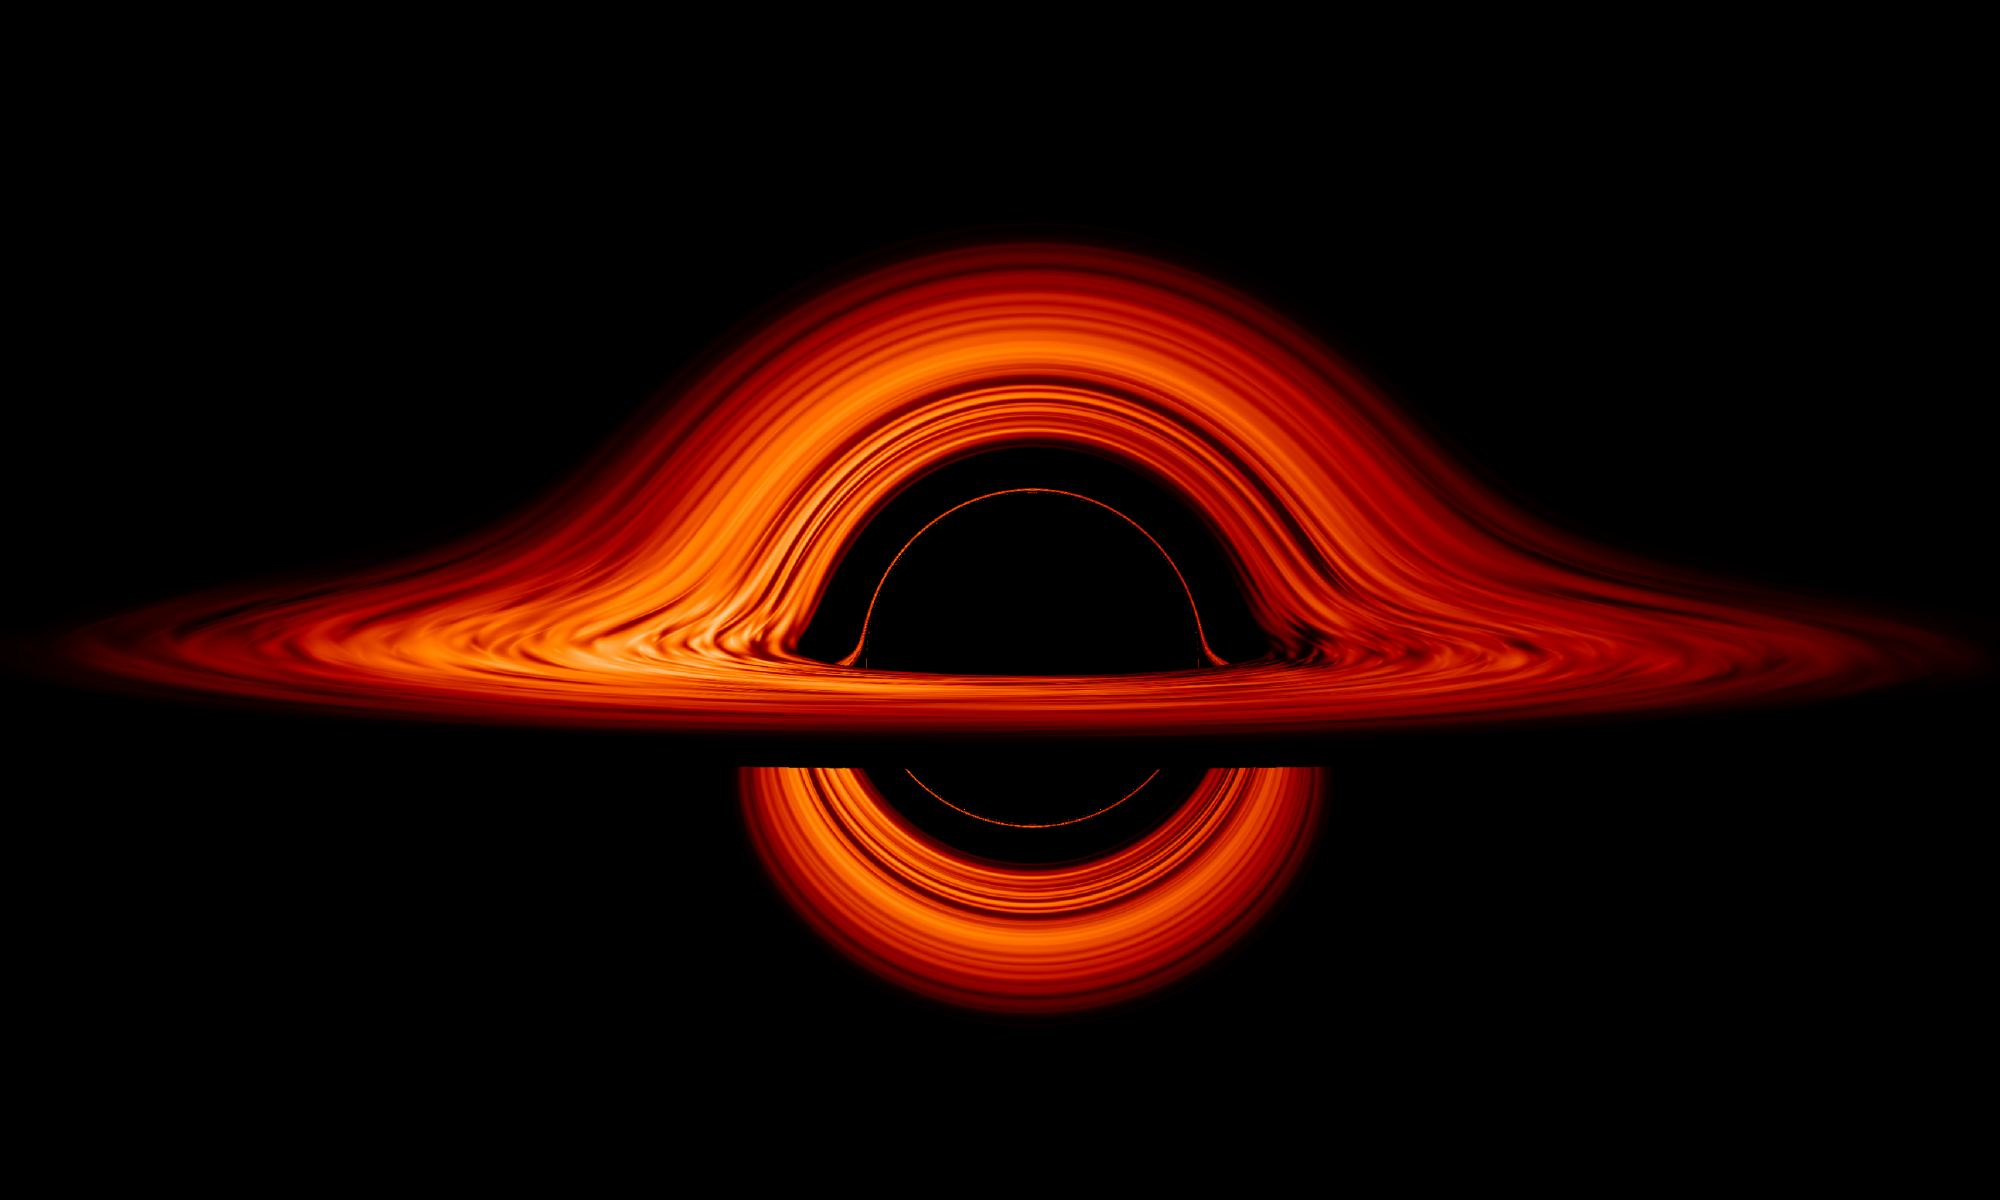
\includegraphics[width=1.0\columnwidth]{img/bh_warped.jpg}
        \caption{Visualization of a black hole accretion disk. The observer's image is warped by extreme gravitational lensing and highly depends on the observer's inclination. Taken from \cite{nasa_img_bh_warped}}
        \label{fig:bh_warped}
    \end{figure}

    As a side note, these simulated images found their way even to a broader audience through pop-cultural references. Professor Thorne himself worked as a science advisor for Christopher Nolan's 2014 movie Interstellar, in which very accurate VFX renders of a supermassive black hole with an accretion disk were used. 

    The other type of sub-Eddington disk that, forms when the opacity is very low, is called ADAF (\emph{Advection-Dominated Accretion Flows}), and it was predicted by \cite{ichimaru1977}. ADAFs are radiatively very inefficient, because the cooling is done dominantly by advection (i.e., heat capture in the matter) and not by radiation. Therefore they are very hot, geometrically extended and more similar in shape tho a sphere than a flat disk \cite{acpow}.

\subsection{Super-Eddington accretion disks}
    Doplnit!!!

    % TODO: doplnit Super-Eddington disky

\subsection[Shakura-Sunyaev $\alpha$-Disc model]{Shakura-Sunyaev $\alpha$-disc}
    \label{sec:alpha_model_definition}
    In 1973, N. I. Shakura and R. Sunyaev proposed an accretion disk model whose source of increased viscosity are the turbulent flow patterns in the disk's body \cite{shakura1973}. This model applies if the modeled system is a \emph{thin disk}, and because of that, it is considered that all material in the disk's body is near its surface, allowing the thermal emission to escape freely. Therefore, self-absorption processes are insignificant. 

    Utilizing equations of hydrostatic equilibrium and Kramer's opacity law on the two-dimensional disk, we can devise a set of equations that describe the local disk structure \cite{acpow}

    \begin{align}
    \begin{split}
        \rho &= \Sigma / H, \\
        H &= c_{\mathrm{s}} R^{3/2} / (GM)^{1/2}, \\
        c_{\mathrm{s}}^2 &= P / \rho, \\
        P &= \frac{\rho k T_{\mathrm{c}}}{\mu m_p} + \frac{4 \sigma}{3 c}T_c^4, \\
        \frac{a \sigma T_{\mathrm{c}}^4}{3 \tau} &= \frac{3GM\dot{M}}{8 \pi R^3}, \\
        \tau &= \Sigma \kappa_{\mathrm{R}}(\rho, T_{\mathrm{c}}) = \tau(\Sigma, \rho, T_{\mathrm{c}}), \\
        \nu \Sigma &= \frac{\dot{M}}{3 \pi} \left[ 1 - \left( \frac{R_*}{R} \right)^{1/2} \right], \\
        \nu &= \nu(\rho, T_{\mathrm{c}}, \Sigma, \alpha, ...).
    \end{split}
    \label{eq:alpha_model_prescription}
    \end{align}

    The set of equations \eqref{eq:alpha_model_prescription} contains eight unknowns: density $\rho$ and temperature $T_{\mathrm{c}}$ of disk's mid-plane, scale height $H$ of the disk, the speed of sound in the medium $c_s$, the sum of gas and radiation pressure $P$, area density $\Sigma$, optical depth $\tau$, and viscosity $\nu$. These unknowns are solved as functions of: accretion rate $\dot{M}$, the central object's mass $M$, the radius of a specific point in the disk $R$, and free parameter $\alpha$. Moreover, $R_*$ represents the radius where angular momentum stops being transported outwards. Assuming that the values $\rho$ and $T_{\mathrm{c}}$ enable the approximation of Rosseland mean opacity using Kramer's law

    \begin{equation}
        \kappa_{\mathrm{R}} = 5 \cdot 10^{24} \rho T_{\mathrm{c}}^{-7/2} \si{\cm^2 \gram^{-1}},
    \end{equation}


    the viscosity of the disk's medium is estimated

    \begin{equation}
        \nu = \alpha c_{\mathrm{s}} H,
    \end{equation}

    where $c_{\mathrm{s}}$ represents the speed of sound in the medium. $H$ represents the scale height of the disk limiting the subsonic turbulent eddies size. The free parameter $\alpha$ ranges between zero (no accretion) and approximately one. Solving the equations \eqref{eq:alpha_model_prescription} with the assumption $\mu = 0.615$ (fully ionized gases), we get a set of relations representing the Shakura-Sunyaev $\alpha$-disc solution \cite{acpow}  

    \begin{align}
    \begin{split}
    \Sigma &= 5.2 \alpha^{-4/5} \dot{M}^{7/10}_{16} m^{1/4}_1 R^{-3/4}_{10} f^{14/5}\ \mathrm{g\ cm^{-2}}, \\
    H &= 1.7 \times 10^8 \alpha^{-1/10} \dot{M}^{3/20}_{16} m^{-3/8}_1 R^{9/8}_{10} f^{3/5}\ \mathrm{cm}, \\
    \rho &= 3.1 \times 10^{-8} \alpha^{-7/10} \dot{M}^{11/20}_{16} m^{5/8}_1 R^{-15/8}_{10} f^{11/5}\ \mathrm{g\ cm^{-3}}, \\
    T_{\mathrm{c}} &= 1.4 \times 10^4 \alpha^{-1/5} \dot{M}^{3/10}_{16} m^{1/4}_1 R^{-3/4}_{10} f^{6/5}\ \mathrm{K}, \\
    \tau &= 190 \alpha^{-4/5} \dot{M}^{1/5}_{16} f^{4/5}, \\
    \nu	&= 1.8 \times 10^{14} \alpha^{4/5} \dot{M}^{3/10}_{16} m^{3/4}_1 R^{3/4}_{10} f^{6/5}\ \mathrm{cm^2\ s^{-1}},  \\
    v_{\mathrm{R}}	&= 2.7 \times 10^{14} \alpha^{4/5} \dot{M}^{3/10}_{16} m^{-1/4}_1 R^{-1/4}_{10} f^{-14/15}\ \mathrm{cm\ s^{-1}},  \\
    \mathrm{with}\ f &= \left[ 1 - \left( \frac{R_*}{R} \right)^{1/2} \right]^{1/4}, \\
    \end{split}
    \label{eq:alpha_model_solution}
    \end{align}

    where $f$ represents the boundary layer function. $\dot{M}_{16}$, $R_{10}$, and $m_1$ are transformed to be represented in typical sizes of disk quantities

    \begin{align}
    \begin{split}
        \dot{M}_{16} &= \dot{M} / 10^{16} \si{\gram \second^{-1}}, \\
        R_{10} &= R / (10^{10} \si{cm}), \\
        m_1 &= M / M_{\odot}.
    \end{split} 
    \end{align}

    Figure \ref{fig:plot_alpha_H_T} shows $T_{\mathrm{c}}$ and $H$ solution examples using different values of free parameter $\alpha$ for the same accretion disk system.

    \begin{figure}[H]
        \centering
        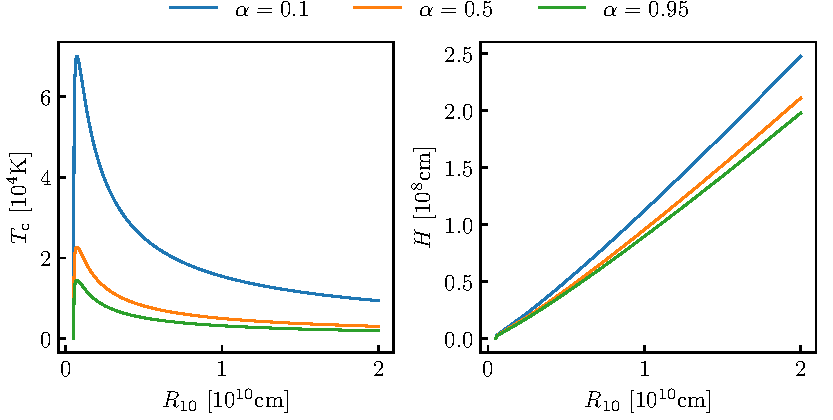
\includegraphics[scale=1.0]{img/plot_alpha_H_T.pdf}
        \caption{$\alpha$-disk model solution examples. Chosen central object's mass is $m_1 = 0.8$. Mid-plane temperatue $T_{\mathrm{c}}$ solution (left) and scale height $H$ (right).}
        \label{fig:plot_alpha_H_T}
    \end{figure}

    
    % 3. CATACLYSMIC VARIABLES
    % \chapter{FLICKERING OF CATACLYSMIC VARIABLES}
\thispagestyle{empty}




    % 4. SIMILARITY OF NON-LINEAR SYSTEMS
    % \chapter{SIMILARITY OF NON-LINEAR SYSTEMS}
\label{chap:similary_of_nonlinear_systems}
\thispagestyle{empty}

% magnetorotacni nestabilita se uvazuje jako pruzina
% msmm je taky pruzina


    % 5. DRIPPING FAUCET
    \chapter{DRIPPING FAUCET}
\label{chap:dripping_faucet}
\mquote{What we know is a drop, what we don't know is an ocean.}{Isaac Newton}
    In the previous chapter, we discussed the possibility of swapping a complex and often computationally demanding model for a simpler alternative that behaves similarly. Because the accretion disk is an incredibly complex system, we must also follow this approach and find a suitable and computationally manageable simplification. We chose to employ a relatively simple model of a dripping faucet, which is a reasonably well-understood system known to exhibit non-linear behavior under certain conditions. There are two types of dripping faucet models. 

    For a better understanding of drop formation processes and a more detailed study of fluid behavior, we can construct a model based on Navier-Stokes equations or Lagrange equations. The key roles in such a model, which is referred to as \emph{Fluid Dynamical Model} (FDM), are played by surface tension, viscosity, and gravity \parencite{faucet1999}.   

    The second type of dripping faucet model is called \emph{Mass-Spring Model}, and as its name suggests, it is based on the approximation of the forming drop as a mass hanging on a spring \citep{shaw1984}. It evolves through time, with the steady fluid influx, until it reaches a predefined critical mass. At that moment, part of the drop is separated, the system resets its parameters, and the cycle repeats. 

    Both types are highly sensitive to the amount of fluid that steadily flows in. This parameter is the determining factor of the non-linear behavior of these systems. Depending on the concrete value of inflow, the dripping intervals can be either periodic or get through period-doubling stages to complete aperiodicity. 

\section{Drop equilibrum states}
    \label{sec:drop_equilibrium_states}
    As a prerequisite for dynamical fluid simulations, we need to know the static equilibrium states of hanging drops on a faucet and evaluate the stability of different shapes and sizes. 

    Let us assume a statically hanging axisymmetrical drop with homogenous fluid density $\rho$. According to \citep{faucet1999}, the drop in equilibrium is defined as follows. The pressure inside the drop is 
    
    % 4.2
    \begin{equation}
        P = \rho g z,
    \end{equation}

    where $z$ represents the vertical coordinate, and $g$ is gravitaional acceleration. The following expression describes the pressure difference between the inside and outside of the drop

    % 4.3
    \begin{equation}
        P = \Gamma \left( \frac{1}{R_1} + \frac{1}{R_2}  \right),
    \end{equation}

    where the surface tension is represented by $\Gamma$. $R_1$ and $R_2$ are the curvature radii of the drop's surface that, for the axisymmetric drop, are

    % 4.5
    \begin{align}
    \begin{split}
        \frac{1}{R_1} &= - \frac{\diff \theta}{\diff s}, \\
        \frac{1}{R_2} &= \frac{\cos \theta}{r}.
    \end{split}    
    \end{align}

    Figure \ref{fig:drop_equilibrum_definition} explains in detail the variables used to calculate the shape of the hanging drop.
    
    \begin{figure}[H]
    \begin{center}
        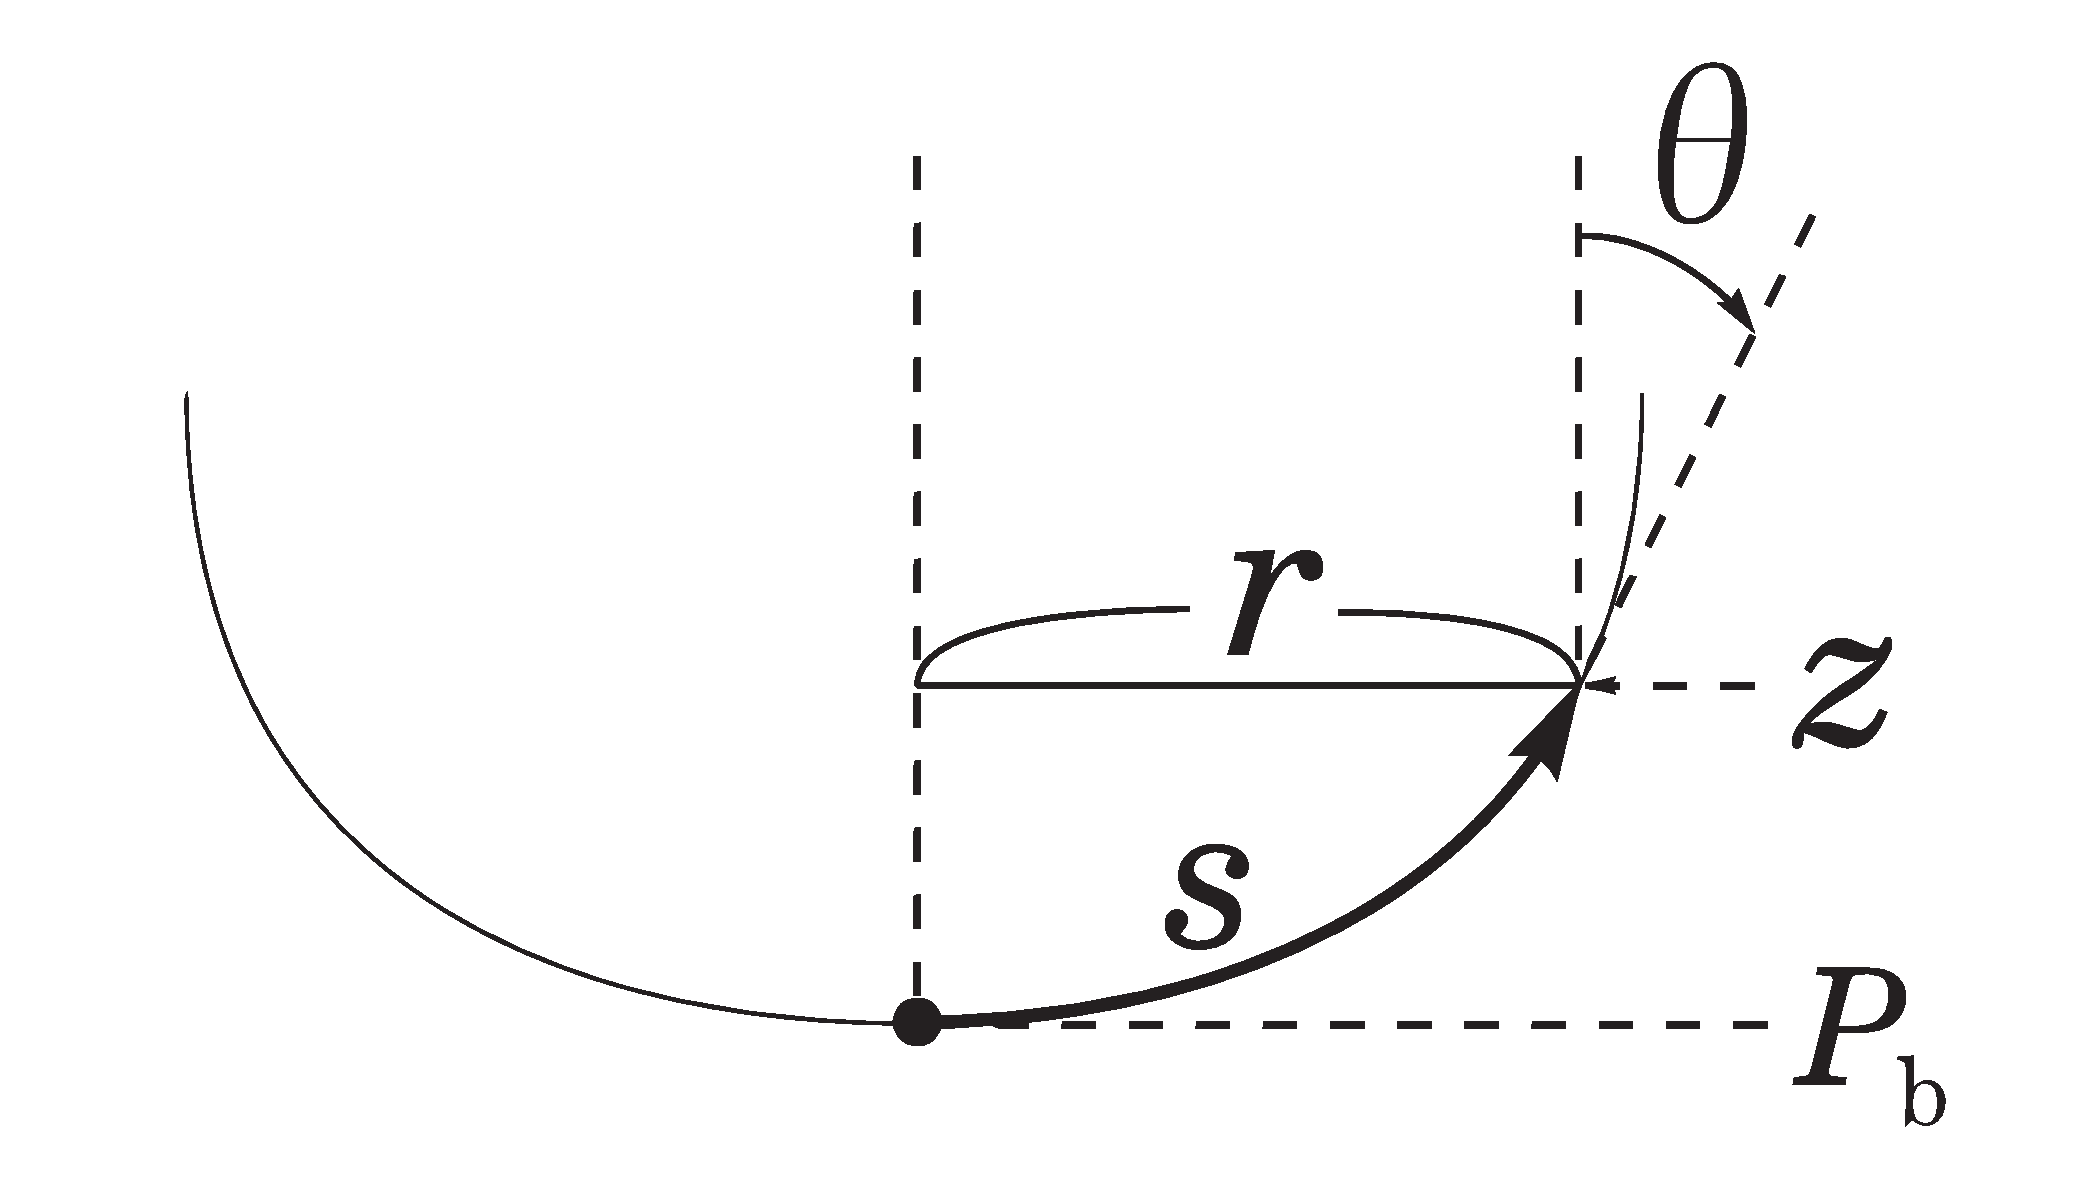
\includegraphics[width=0.75\columnwidth]{img/drop_equilibrum_definition.pdf}
    \end{center}
    \caption{Definition of variables for the hanging drop system. Taken from \citep{faucet1999}} 
    \label{fig:drop_equilibrum_definition}
    \end{figure}

    % 4.4
    \begin{align}
    \begin{split}
        m_0 &= \rho l_0^3 = 0.02 \si{\gram}, \\
        P_0 &= \sqrt{\rho g \Gamma} = 270 \si{dyne \cdot \cm^{-2}}, \\
        l_0 &= \sqrt{\frac{\Gamma}{\rho g}} = 0.27 \si{\cm}, \\
        t_0 &= 0.017 \si{\second}.
    \end{split}
    \label{eq:base_units_drop}
    \end{align}

    Defined by equations \eqref{eq:base_units_drop} are the base units of mass, pressure, and length, that sets $\Gamma = \rho = g = 1$; assuming the medium is water at $20 \si{\celsius}$. The drop's shape is then described by a set of ODE's \eqref{eq:drop_equilibrum_odes}, that are solved numerically, with the use of the initial conditions: $z(0) = P_{\mathrm{b}}$, $\theta(0) = \pi / 2$, and $r(0) = 1 \cdot 10^{-20}$

    % 4.6
    \begin{align}
    \begin{split}
        \frac{\diff r}{\diff s} &= \sin \theta, \\
        \frac{\diff z}{\diff s} &= - \cos \theta, \\
        \frac{\diff \theta}{\diff s} &= \frac{\cos \theta}{r} - z.
    \end{split}
    \label{eq:drop_equilibrum_odes}
    \end{align}

    Figure \ref{fig:plot_drop_equilibrium_ceiling} shows multiple equilibrium state solutions for different values of pressure $P_{\mathrm{b}}$ at the bottom of the drop.

    \begin{figure}[H]
    \begin{center}
        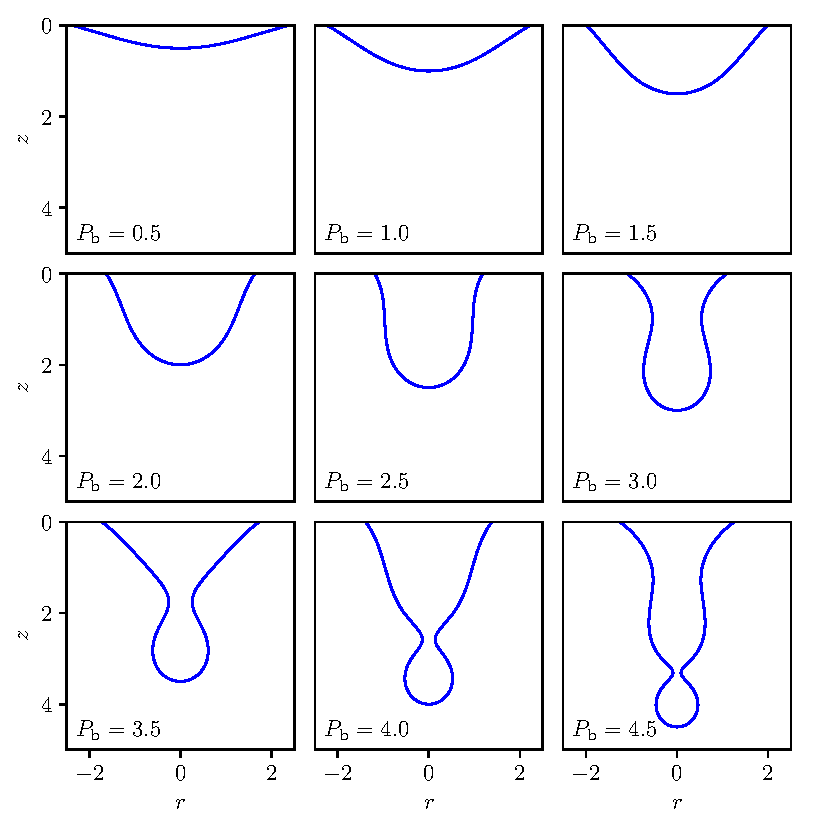
\includegraphics[width=1.0\columnwidth]{img/plot_drop_equilibrium_ceiling.pdf}
    \end{center}
        \caption{Examples of unbounded static equilibrium drop states, which are solutions of ODE's \eqref{eq:drop_equilibrum_odes} for different values of pressure $P_{\mathrm{b}}$ on the bottom of the drop.}
    \label{fig:plot_drop_equilibrium_ceiling}
    \end{figure}
    
    Similarly to solutions shown in Figure \ref{fig:plot_drop_equilibrium_ceiling}, we can bound the equilibrium states to a faucet of chosen radius $r_{\mathrm{a}}$. This is done by using the same solutions, finding a point of the closest match with the chosen boundary (i.e., the faucet), and shifting $z$ coordinates accordingly. Figure \ref{fig:plot_drop_equilibrium_faucet} shows drop solutions bounded to a faucet. Both unbounded and bounded examples are done for the same initial conditions. 

    \begin{figure}[H]
    \begin{center}
        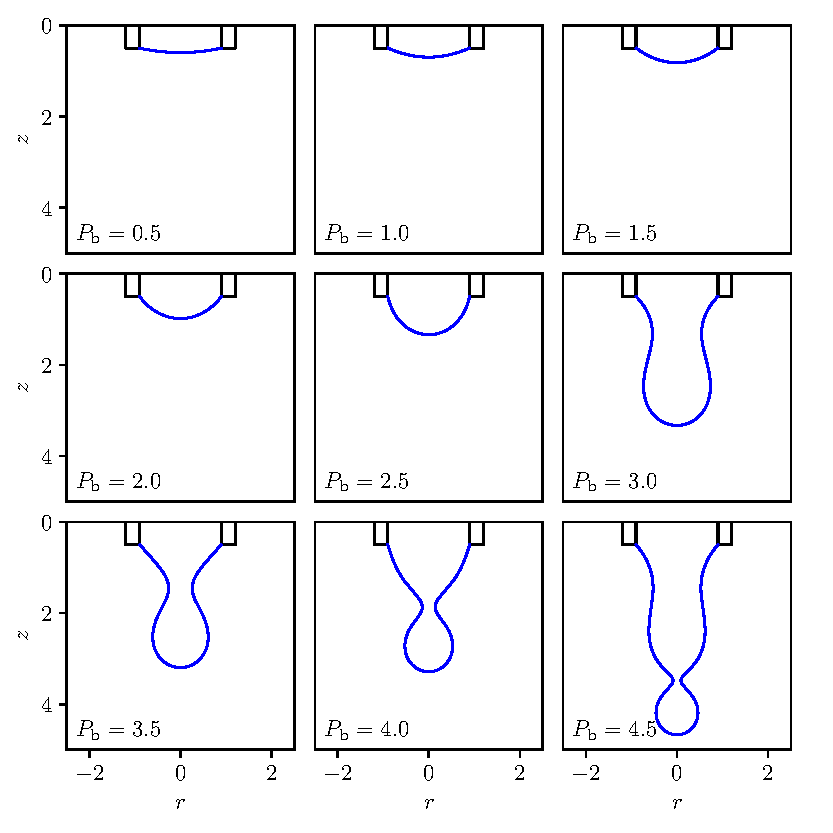
\includegraphics[width=1.0\columnwidth]{img/plot_drop_equilibrium_faucet.pdf}
    \end{center}
        \caption{Examples of static equilibrium drop states bounded to a faucet, which is solutions of ODE's \eqref{eq:drop_equilibrum_odes} for different values of pressure $P_{\mathrm{b}}$ on the bottom of the drop.}
    \label{fig:plot_drop_equilibrium_faucet}
    \end{figure}

    We assume, as is also self-evident from Figures \ref{fig:plot_drop_equilibrium_ceiling} and \ref{fig:plot_drop_equilibrium_faucet}, that not all of these solutions are stable and therefore usable as initial states of FDM. \emph{Stable}, in this sense, means that the drop shape (i.e., particular solution) stays statically hanging on the faucet, assuming there is no fluid inflow. We can distinguish the stable and unstable solutions based on the relation between drop' volume $V_{\mathrm{d}}$ and the pressure $P_{\mathrm{b}}$ 

    \begin{equation}
        V_{\mathrm{d}} = f(P_{\mathrm{b}}) 
    \end{equation}

    \begin{figure}[H]
    \begin{center}
        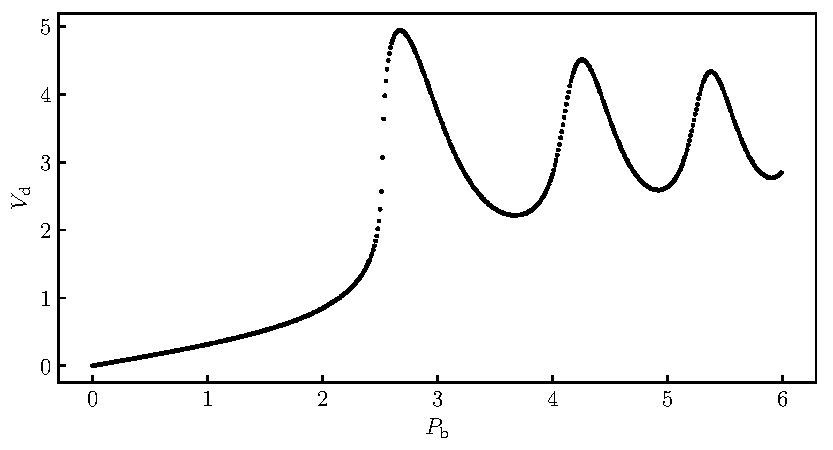
\includegraphics[width=1.0\columnwidth]{img/plot_drop_equilibrium_faucet_pv.pdf}
    \end{center}
        \caption{Static equilibrium solutions of drop shapes hanging on a faucet or radius $r_{\mathrm{a}} = 0.952$. Every point of the solutions curve represents one solution in the interval $P_{\mathrm{b}} \in \langle 1 \cdot 10^{-20}, 6.0 \rangle$.} 
    \label{fig:plot_drop_equilibrium_faucet_pv}
    \end{figure}
        

    As shown by \citep{padday1973}, there is only one stable solution for a given value of the drop's volume. Figure \ref{fig:plot_drop_equilibrium_faucet_pv} demonstrates that for different initial values of $P_{\mathrm{b}} \in \langle 1 \cdot 10^{-20}, 6.0 \rangle$, there are multiple solutions of the same drop's volume. Only the solutions in the interval

    \begin{equation}
        P_{\mathrm{b}} \in \langle 1 \cdot 10^{-20}, 2.67 \rangle,
    \end{equation}

    are the stable ones. Solutions shown in Figure \ref{fig:plot_drop_equilibrium_faucet_pv} are all done assuming the boundary to a faucet with radius $r_{\mathrm{a}}$. This interval of stable drop shapes also provides us with the maximum stable volume of the hanging drop for a particular faucet radius. In the case of $r_{\mathrm{a}} = 0.952$ the maximum stable volume is $V_{\mathrm{d}} = 4.95$.

\section{Fluid dynamical model (FDM)}
    The theory behind drop formation and breakup is a surprisingly recent invention, even though it concerns an everyday phenomenon. However, J. Eggers' scaling theory is universally applicable for viscous axisymmetrical drop formation \citep{eggers1993}, which was later used as a basis for dynamical drop simulations done by \citep{faucet1999}. In the following sections, we will go over the process of modeling the process of FDM. Although this more complex dripping faucet model is more suitable for studying short-term behavior and detailed shapes of forming drops, it is also a precursor for a better understanding the spring-like MSM models discussed later in this chapter.

\subsection{Diskretized FDM Lagrangian}
    The starting point of the simulation is the drop shape in the state of equilibrium (see Section \ref{sec:drop_equilibrium_states}); in particular, the equilibrium solution with the highest stable drop volume $V_{\mathrm{d}}$ for the chosen faucet radius $r_{\mathrm{a}}$. The reason is that as we add more fluid to the system, its path to reaching the critical mass, and therefore the drop breakup, will be the shortest.

    Let us start by defining the Lagrangian for the drop system
    
    % 4.9
    \begin{equation}
        \mathcal{L} = E_{\mathrm{k}} - U_{\mathrm{g}} - U_{\Gamma},
    \end{equation}

    where $E_{\mathrm{k}}$ represents the total kinetic energy of the drop, $U_{\mathrm{g}}$ its total potential energy and $U_{\Gamma}$ its total surface energy. Discretization of the system is done by splitting the drop into $M$ number of disks with equal length along drops surface $\Delta s$ (see. Figure \ref{fig:drop_equilibrum_definition}). The disk has a mass

    \begin{equation}
        m_j = \rho \Delta \xi_j,
    \end{equation}

    where $\Delta \xi_j$ is the volume of particular disk. Because the fluid density is defined as $\rho = 1$, the mass of a single disk is simply

    \begin{equation}
        m_j \equiv \Delta \xi_j.
    \end{equation}

    Therefore the total kinetic energy of the drop system expressed as a sum of individual disks is 

    %4.10
    \begin{equation}
        E_{\mathrm{k}} = \frac{1}{2} \sum^M_{j=1} \Delta \xi_j \dot{z}_j^2.
    \end{equation}

    Similarly, the potential energy is a sum of its values for all disks

    %4.11
    \begin{equation}
        U_{\mathrm{g}} = -g \sum^M_{j=1} \Delta \xi_j z_j,
    \end{equation}

    where $g$ is the gravitational acceleration. The expression for surface energy is approximated by 

    %4.12
    \begin{equation}
        U_{\Gamma} = \Gamma S,
    \end{equation}

    where $S$ represents the total surface area of the drop. The computation of the surface energy comes down to determining the surface area $S$ as a sum of individual disk surfaces. We can approximate the surface area $S_j$ of a single disk as the surface area of the truncated cone's outer shell in the interval $\langle (z_{j+1} + z_j) / 2; (z_j + z_{j-1}) / 2 \rangle$, which then is

    %4.13
    \begin{equation}
        S_j = \pi (r_j + r_{j+1}) \sqrt{\frac{1}{4} (z_{j+1} - z_{j-1})^2 + (r_j - r_{j+1})^2}.
    \end{equation}

    Assuming the average radii of disks
    
    %4.18
    \begin{equation}
        r_j = \sqrt{\frac{\Delta \xi_j}{\pi (z_j - z_{j-1})}}.
    \end{equation}

    Therefore the surface energy is then expressed as

    \begin{equation}
        U_{\Gamma} = \Gamma \sum_{j=1}^M S_j(z_{j-1}, z_j, z_{j+1}),
    \end{equation}

    which gives us the final Lagrangian of the discretized drop system

    \begin{equation}
        \mathcal{L} = E_{\mathrm{k}}(\dot{z}_1, ..., \dot{z}_M) - U_{\mathrm{g}}(z_1, ..., z_M) - U_{\Gamma}(z_1, ..., z_M)
    \end{equation}

    To conduct the simulation, the equations of motion for the drop system are calculated from

    \begin{equation}
        \frac{\diff}{\diff t} \frac{\partial \mathcal{L}}{\partial \dot{z}_j} = \frac{\partial \mathcal{L}}{\partial z_j} + \frac{1}{2} \frac{\partial \dot{E}_{\mathrm{k}}}{\partial \dot{z}_j}
    \end{equation}

    where $\mathcal{L}$ is the previously obtained Langrangian of the drop as a sum of its disk discretization in the interval $j \in \langle 1; M \rangle$. Examples of the simulation results done by \citep{faucet1999} are shown in Figure \ref{fig:plot_fdm_simulation}.
    
    \begin{figure}[H]
    \begin{center}
        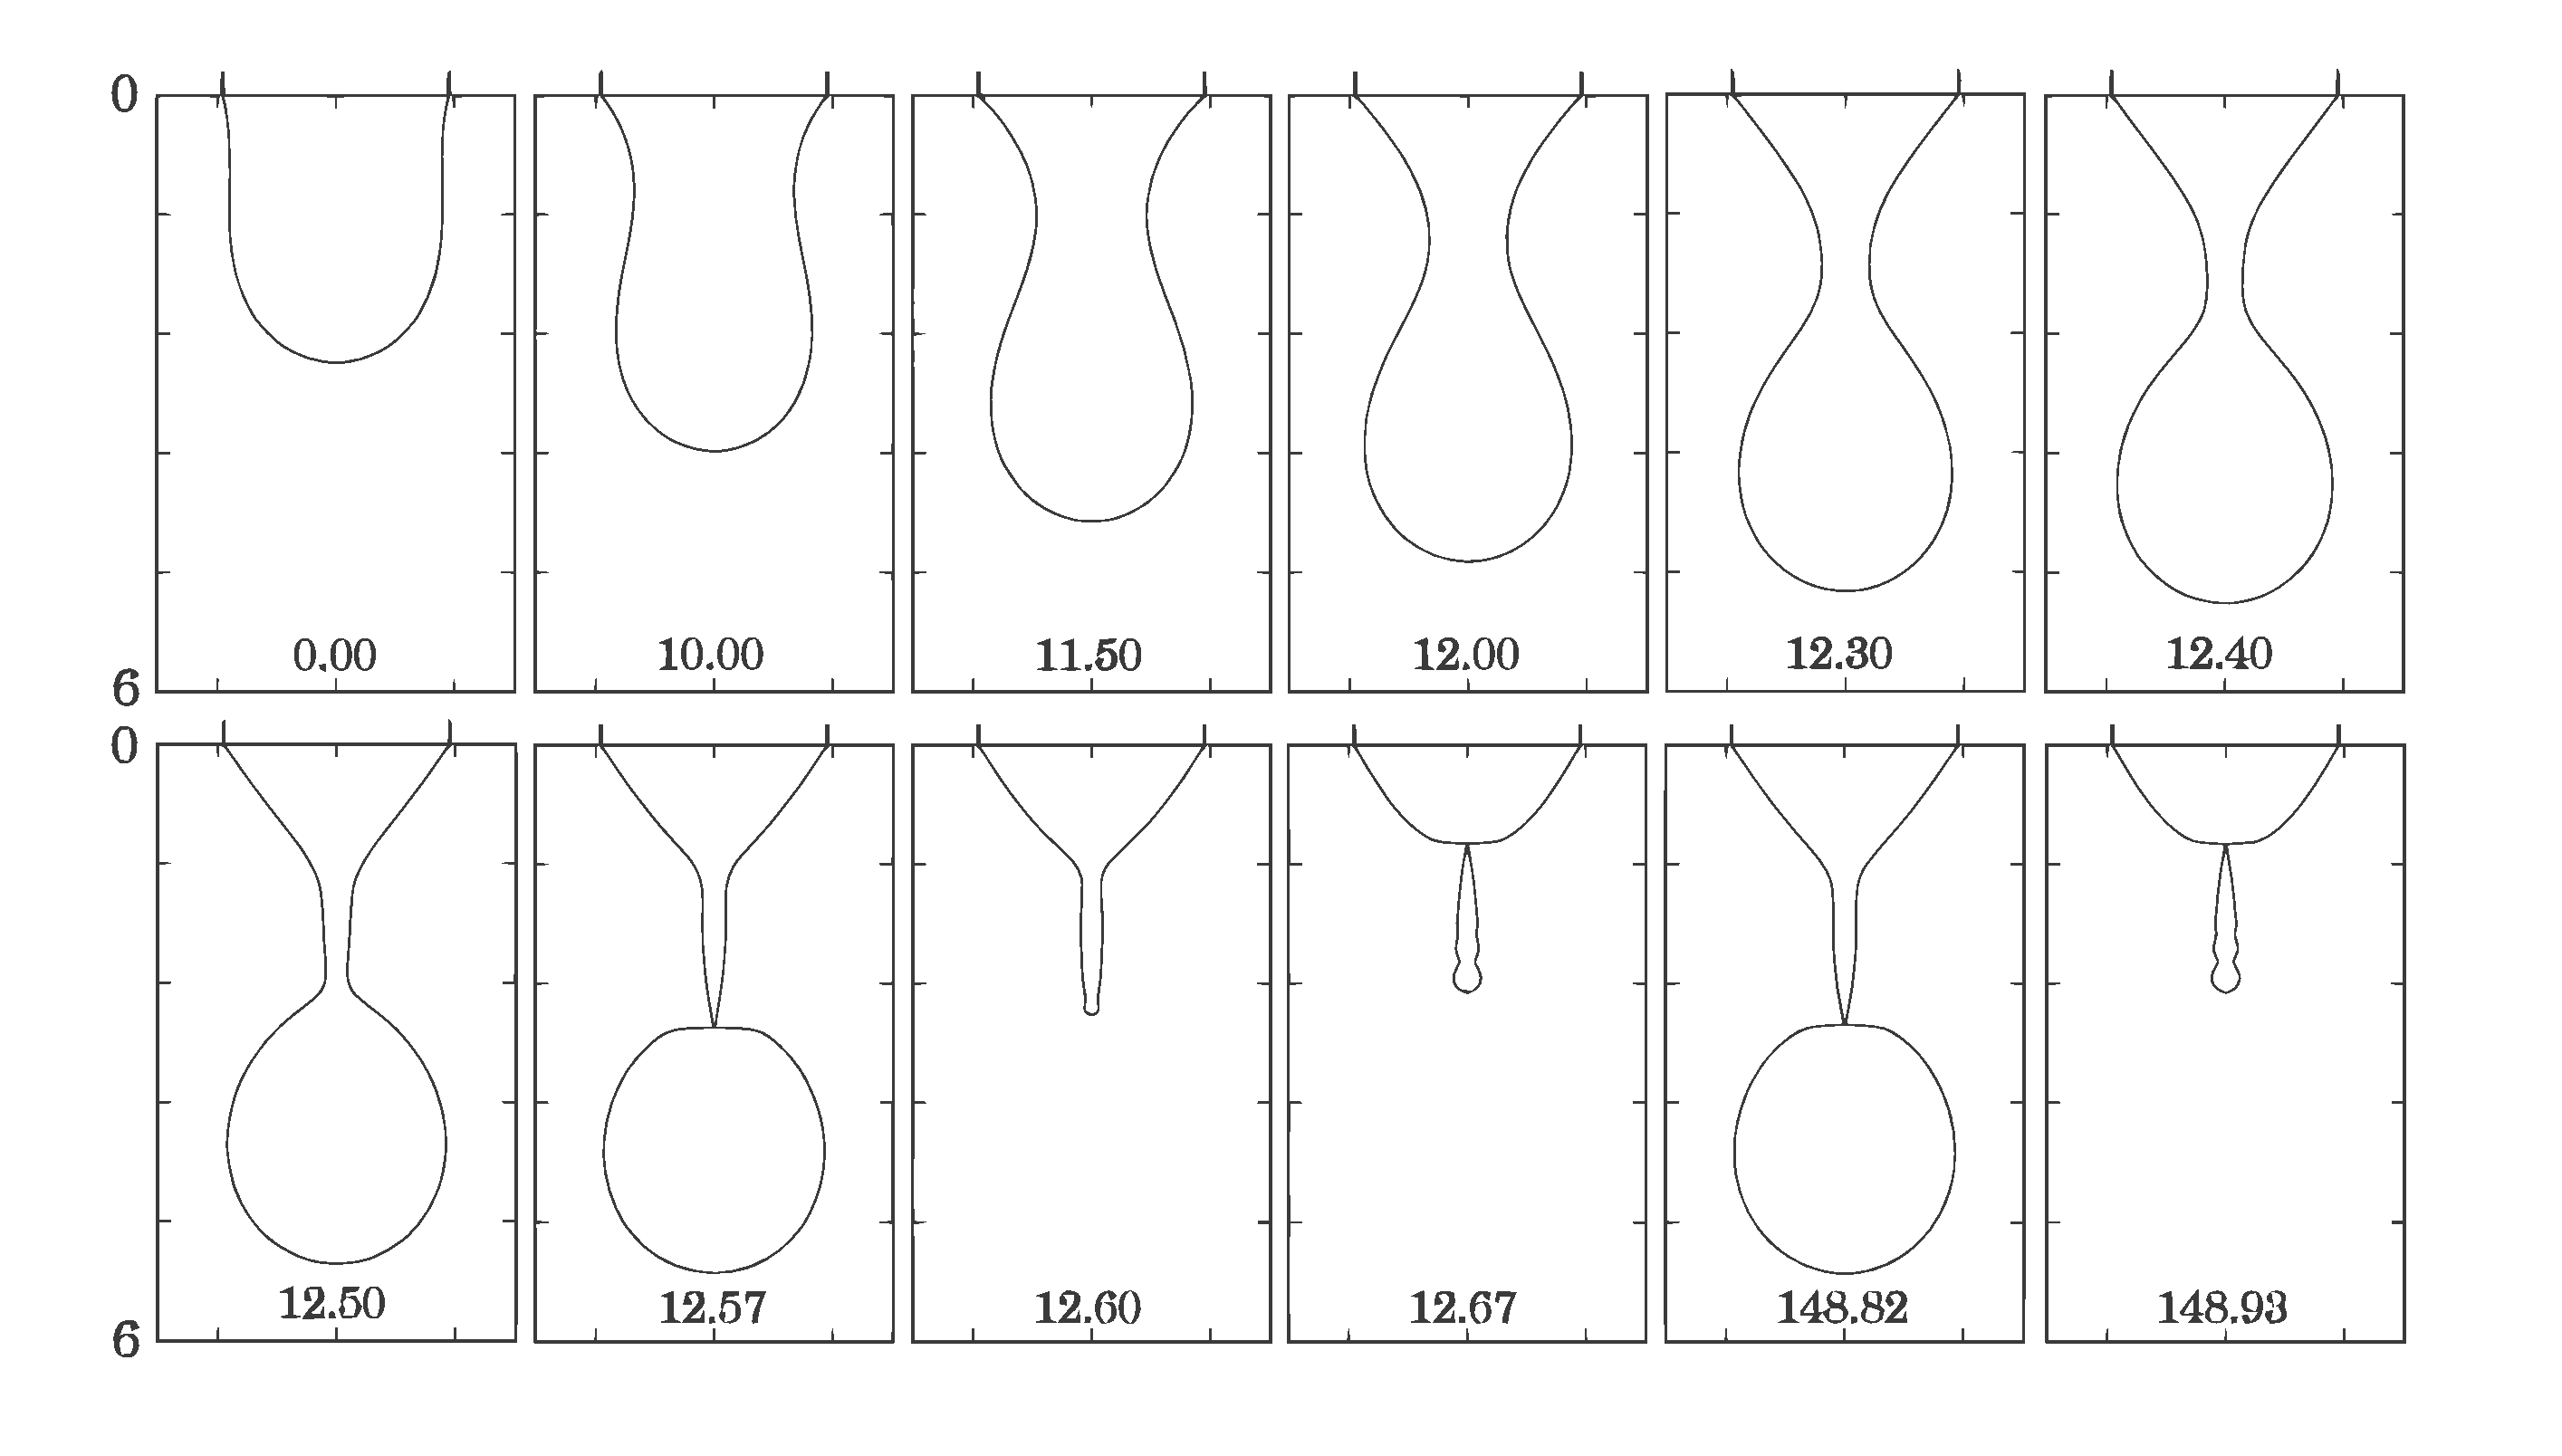
\includegraphics[width=1.0\columnwidth]{img/plot_fdm_simulation.pdf}
    \end{center}
        \caption{Time development of drop shape for the faucet radius $r_{\mathrm{a}} = 0.952$. Taken from \citep{faucet1999}.}
    \label{fig:plot_fdm_simulation}
    \end{figure}

\section{Mass-spring model (MSM)} 
    \label{section:msm}

    The less complex counterpart to the \emph{Fluid Dynamical model} is the \emph{Mass-Spring model}, which is more suitable for studying the long-term behavior of the dripping faucet system. This model was first proposed by \citep{shaw1984} and later modified by \citep{msmm1999}. The forming drop on a faucet is modeled using a one-dimensional spring system with variable stiffness $k$ and a mass $m$ attached. As the simulation progresses, the spring elongation $z$ (i.e., the position of hanging mass) is monitored. If the critical value of elongation $z_{\mathrm{c}}$ is reached, the predefined part of the drop breaks out, the system parameters reset, and the cycle continues.

    The original version defined by \citep{shaw1984} is described by a set of ODE's 

    \begin{align}
    \begin{split}
        \D{}{t} \left(m \D{z}{t}\right) &= -kz - \gamma\D{z}{t} + mg, \\
        \D{m}{t} &= Q,
    \end{split}
    \label{eq:msm_original_odes}
    \end{align}

    where $z$ represents the spring elongation, $m$ mass of the hanging drop. The constant damping ratio is $\gamma = 0.05$, $Q$ represents the constant mass inflow from the faucet, and the spring stiffness $k$, depending on the current mass of the drop, is defined as
    
    \begin{equation}
        \begin{aligned}
            & k~=
            \begin{cases}
                -11.4\ m + 52.5 \hspace{10mm} (m < 4.61) \\
                \hspace{14.5mm} 0 \hspace{20mm} (m \ge 4.61 ).
            \end{cases}
        \end{aligned}
        \label{eq:spring_stiffness}
    \end{equation}
    
    Relations expressed by \eqref{eq:spring_stiffness} and the value of $\gamma$ were obtained experimentally by \citep{shaw1984} and provide a good description for the real-world behavior of drops and leaky faucets.

    Based on \eqref{eq:msm_original_odes}, \citep{msmm1999} proposed an improved version of MSM that is expressed by following set of ODE's

    \begin{align}
    \begin{split}
        \D{p}{t} &= -kz - \gamma\D{z}{t} + mg, \\
        \D{p}{t} &= m \frac{\diff^2 z}{\diff t^2} + \left(\D{z}{t}  \right)\D{m}{t}.
    \end{split}
    \label{eq:msm_original_moded_odes}
    \end{align}

    Equations \eqref{eq:msm_original_moded_odes} are then converted to a form suitable for numerical solution by an appropriate method (e.g., methods from the Runge-Kutta family)
    
    %4.33
    \begin{align}
    \begin{split}
        \dot{z} &= v \\
        \dot{v} &= g - \frac{1}{m}[kz + \gamma v + (v - v_0)Q]
    \end{split}
    \end{align}

    where $Q$ is the inflow to the faucet, that is defined as

    %4.31
    \begin{equation}
        \D{m}{t} = Q = \pi r_{\mathrm{a}}^2 v_0.
    \end{equation}

    The value $v_0$ represents the fluid flow velocity from the faucet, which is a constant value. By choosing different velocities $v_0$, we can drastically alter the system's behavior, from periodic through period-doubling stages to complete aperiodicity. 

    An important aspect of the simulation is, monitoring the critical value of elongation $z_{\mathrm{c}}$. The drop breaks out when the condition is met and model parameters are reset. The precise value of $z_{\mathrm{c}}$ according to \citep{msmm1999} is
    
    \begin{equation}
        z_{\mathrm{c}} = 5.5.
        \label{eq:z_critical_model}
    \end{equation}

    The amount of mass $m_r$ that remains on the faucet after the breakup is
    
    \begin{equation}
        m_{\mathrm{r}} = 0.2 m + 0.3,
    \end{equation}

    which is also an experimentally obtained relation that corresponds well with observations of real dripping faucets. As a demonstration, we have done many simulations for the same arbitrary faucet radius $r_{\mathrm{a}} = 0.916$, with the individual simulation with different inflow velocity in the interval $v_0 = \langle 0.13; 0.18 \rangle$, and velocity value increment $\Delta v_0 = 5.0 \cdot 10^{-5}$. One result example for $v_0 = 0.146$ plotted as projections of phase space is shown in Figure \ref{fig:plot_msm_state_space}. 

    \begin{figure}[H]
    \begin{center}
        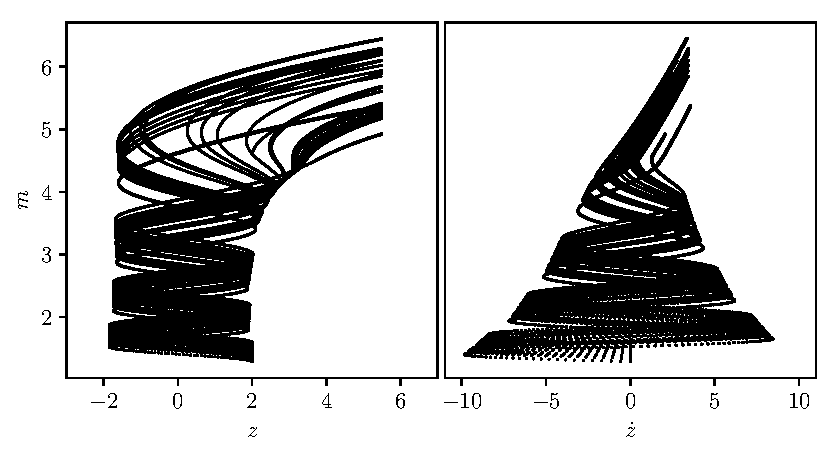
\includegraphics[width=1.0\columnwidth]{img/plot_msm_state_space.pdf}
    \end{center}
        \caption{Phase space portrait projections of MSM, where \mbox{$r_{\mathrm{a}} = 0.916$}, $v_0 = 0.146$.}
    \label{fig:plot_msm_state_space}
    \end{figure}

    A good demonstration of the non-linear behavior of the MSM system is the bifurcation diagram, which is constructed by plotting the periods between two consecutive drop breakups $T_n$ in relation to the inflow velocity $v_0$. For example, in the bifurcation diagram shown in Figure \ref{fig:plot_msm_bifurcation}, we can see inflow velocity intervals of periodic dripping and total aperiodic behavior. 

    \begin{sidewaysfigure}
        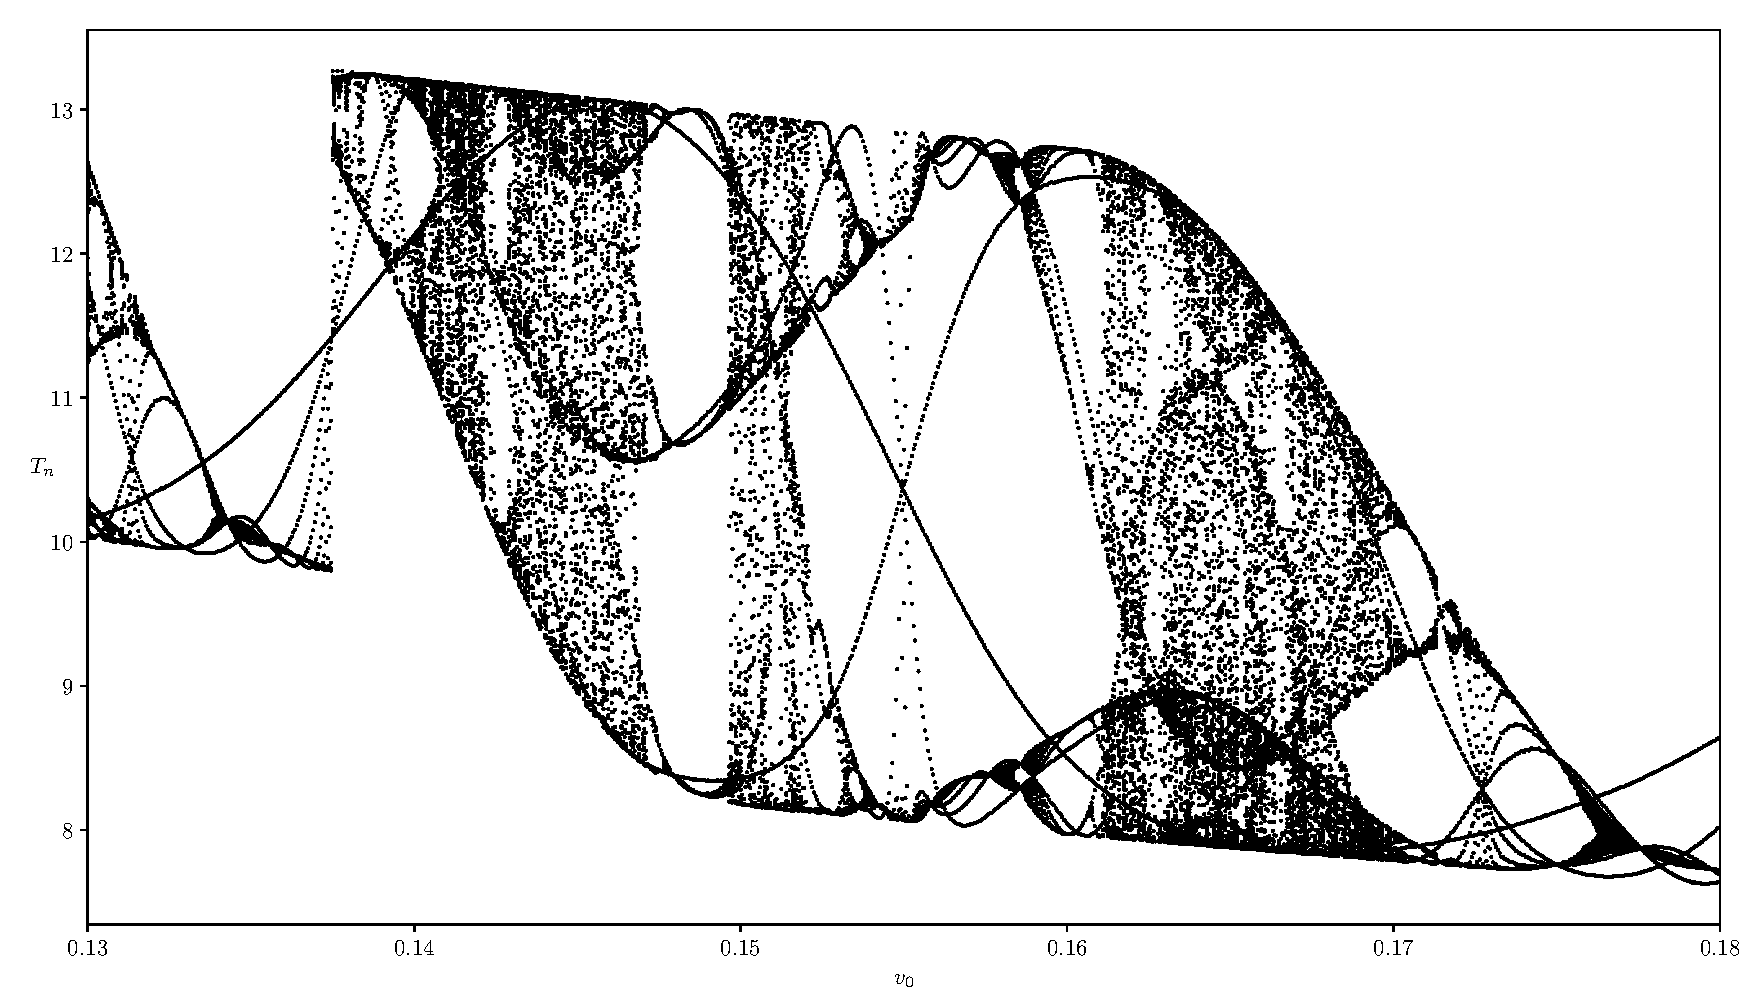
\includegraphics[width=1.0\columnwidth]{img/plot_msm_bifurcation.pdf}
        \caption{Bifurcation diagram of MSM in the }
        \label{fig:plot_msm_bifurcation}
    \end{sidewaysfigure}

% TODO: sekce o "Dripping Handrail" modelech
% \section{Dripping handrail models}




    % 6. MDH - MODEL DEFINITION 
    \chapter{MULTILAYER DRIPPING HANDRAL}
    \label{chap:multilayer_dripping_handrail}
    \thispagestyle{empty}
    \mquote{Essentially, all models are wrong, but some are useful.}{George E. P. Box}

    As discussed in Chapter \ref{chap:similary_of_nonlinear_systems}, some models of physical systems can be very computationally demanding, so a simpler and manageable model analogy is often needed. For example, if we wanted to simulate the accretion disk system without simplification, it would be almost impossible to compute in the authors' lifetime. Such a model would be composed of individual and interacting gas particles. It would require either plasma physics equations or Navier-Stokes equations with a magnetic field; at that point, it is not a model but a perfect analogy. 

    The model developed for this study provides a manageable and reasonably complex tool for accretion disk simulation. Based upon its apparent characteristics, we call it \emph{Multilayer Dripping Handrail} (MDH) because it is an arrangement of concentric rings (i.e., layers). Each layer consists of up to several hundred cells, and each behaves as a \emph{dripping faucet}. The dripping mechanism drives the distribution of matter through the layers until they reach the central object.

% ---------
% The Model
% ---------
\section{The model}
    The MDH model is inspired by the model created by \citep{yonehara1997}. However, our model takes this concept much further. Instead of a simple mass limit condition, we use a slightly modified implementation of the Mass-Spring model (MSM) as a means of non-linear matter redistribution. We discussed the original MSM in detail in Chapter \ref{chap:dripping_faucet}. 

\subsection{The cellular accretion disk model}
    The concept of cellular automaton (CA) is quite an old idea in computer science that Stanislaw Ulam and John von Neuman first discovered at Los Alamos National Laboratory. However, it gained wider popularity after the publishing of \emph{Conway's Game of Life} \citep{gardner1970} and also extensive studies done by Stephen Wolfram starting in the 1980s.

    CA definition provided by \citep{wolfram2002} states that: \emph{Cellular automaton is a collection of cells on a grid of specified shape that evolves through a number of discrete time steps according to a predefined set of rules based on neighboring cells.} In our case, this set of rules mainly deals with distributing matter between the cells and throughout the accretion disk body.

    MDH is a cellular automaton that arranges $I$ times $J$ cells in a concentric ring (i.e., layers) grid pattern. The layers a denoted by 

    \begin{equation}
        i \in [0;I-1].
    \end{equation}

    The layer $i=0$ represents the outer edge layer of the disk. Each layer contains $J$ individual cells denoted by

    \begin{equation}
        j \in [0;J-1].
    \end{equation}

    Because the orbital angular velocities of individual layers differ, the simulation grid naturally shifts over time. Figure~\ref{fig:grid_states} demonstrates the possible simulation grid states. On the left, we see the non-shifted initial state of the simulation. On the right, the layers of cells are slightly shifted after an arbitrary number of simulation steps.

    \begin{figure}[H]
    \centering
    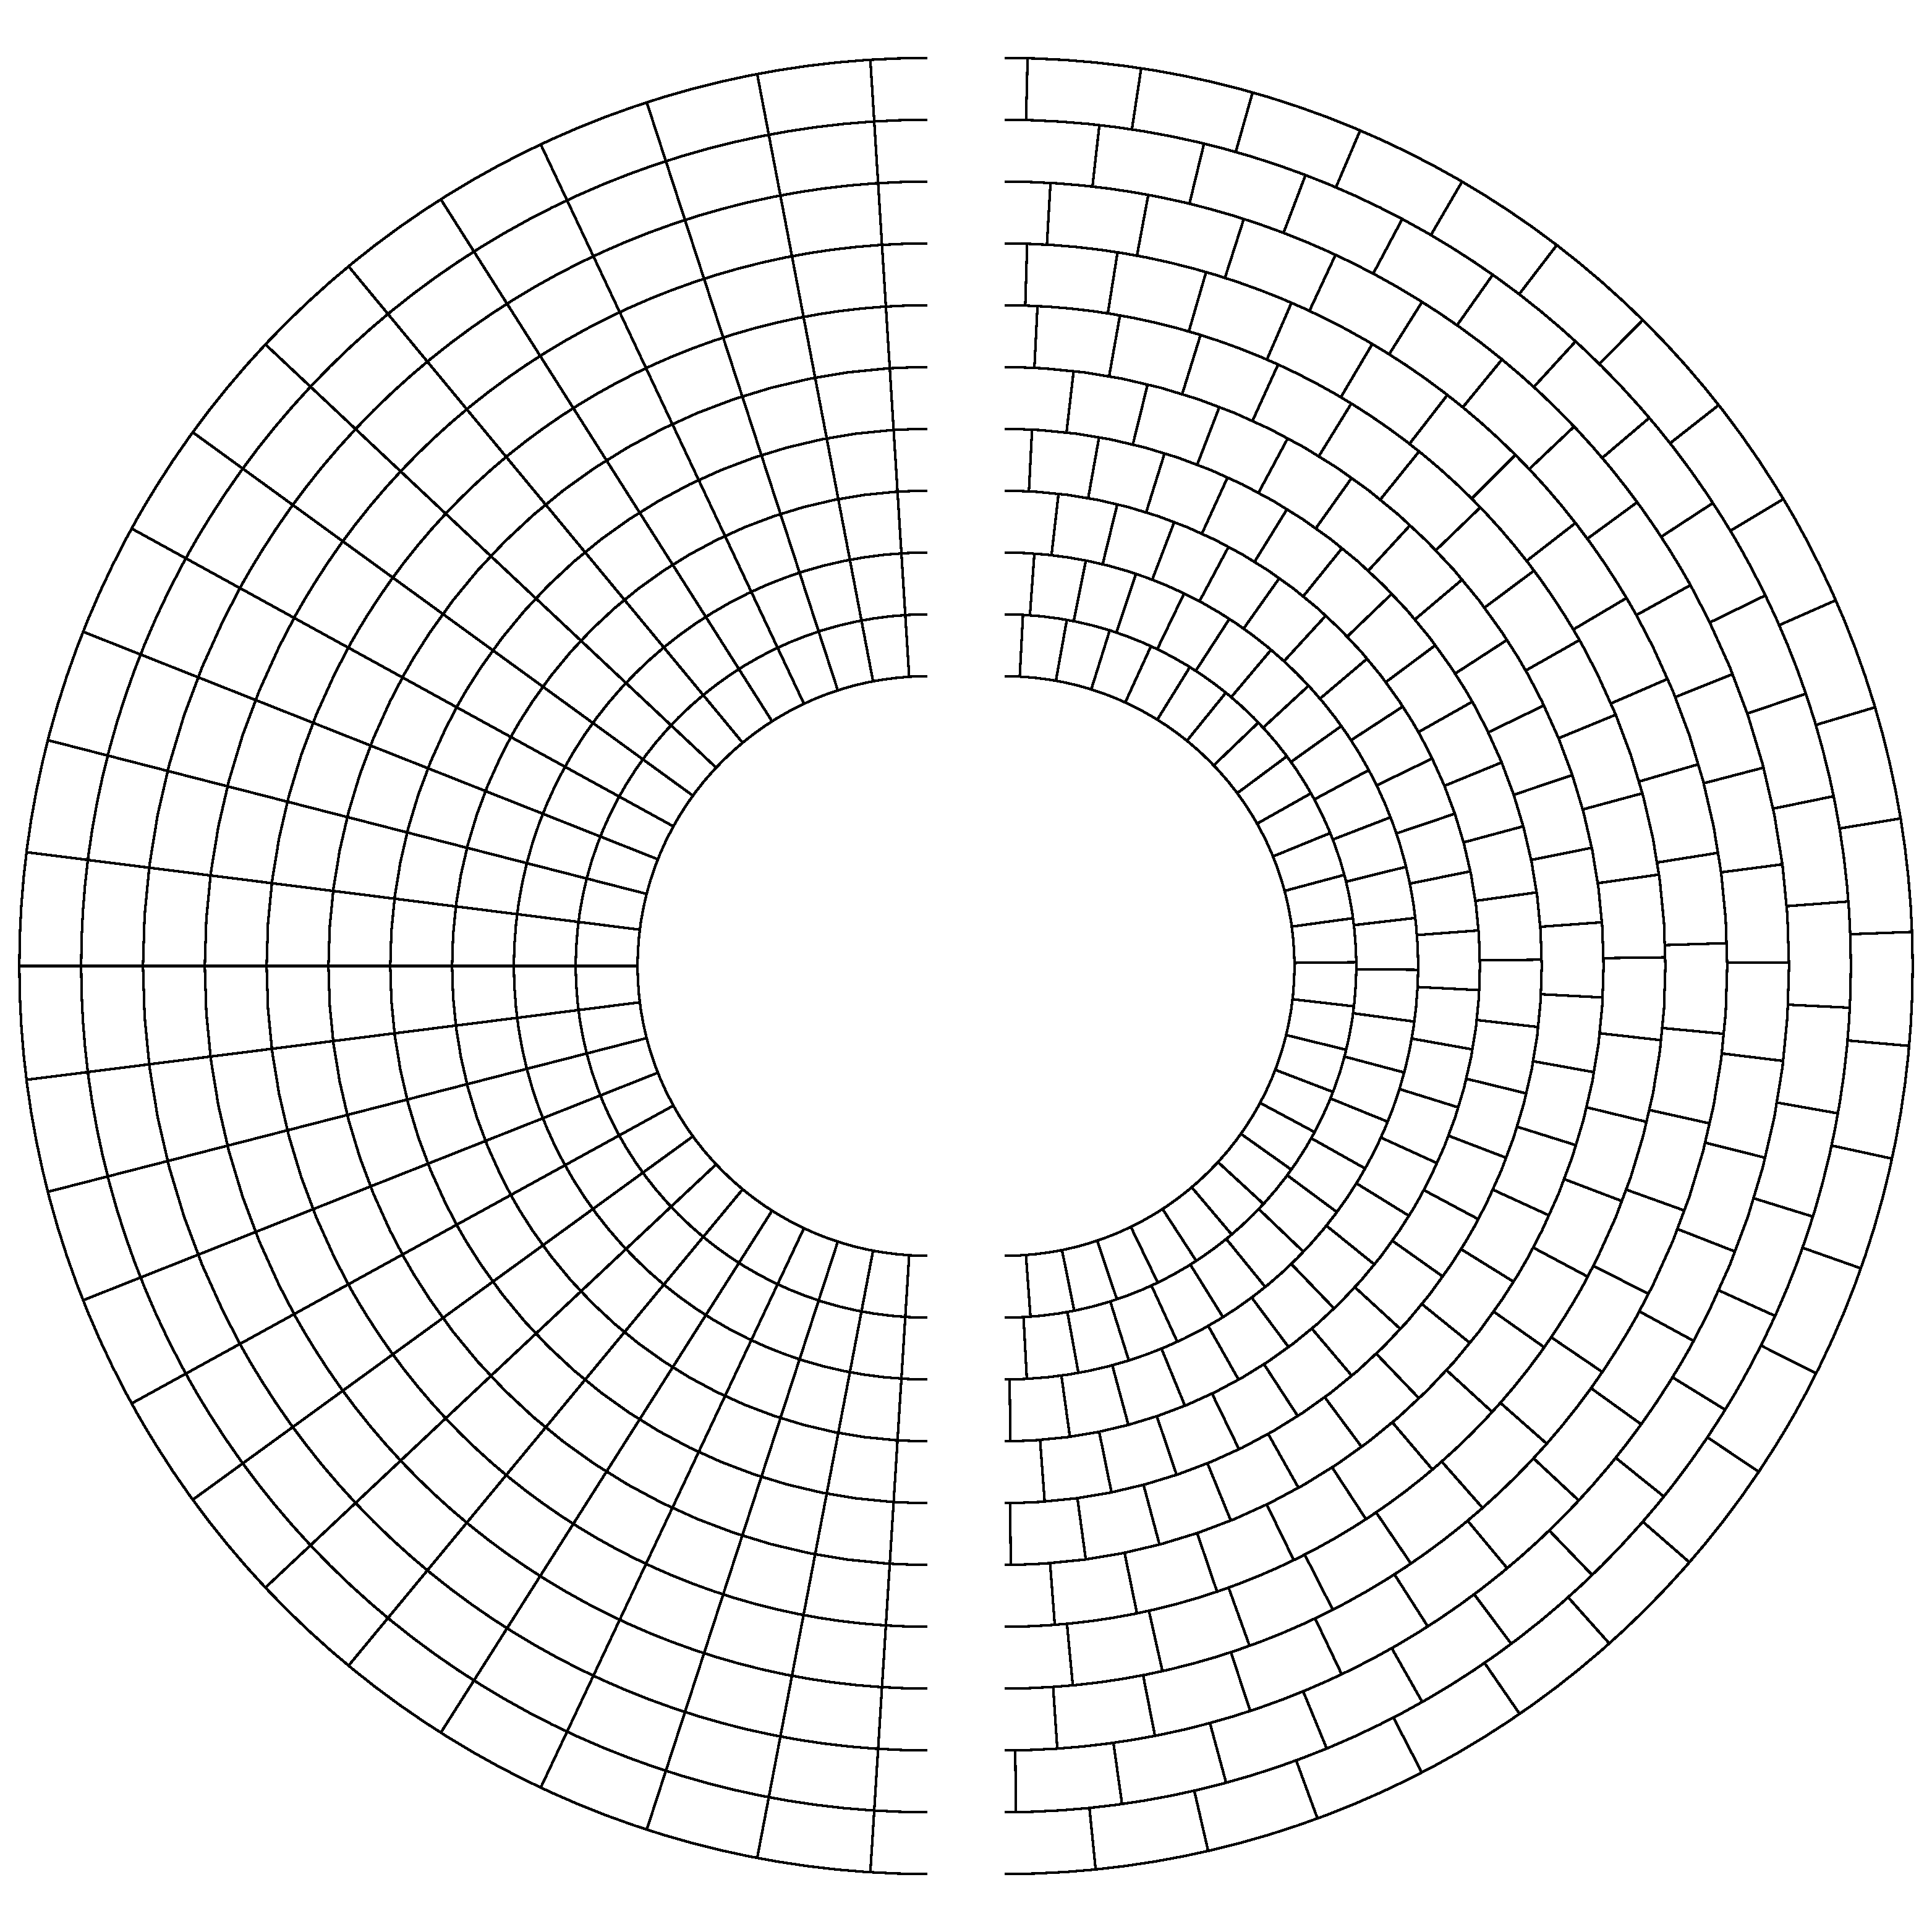
\includegraphics[width=\columnwidth]{img/grid_states.pdf}
    \caption{Grid states. Initial grid state (left) and shifted state after some arbitrary number of simulation steps (right).}
    \label{fig:grid_states}
    \end{figure}

    In the original MSM defined by \eqref{eq:msm_original_odes}, gravitational acceleration is a constant value. In our modification, it is substituted by $f_g$. We call this layer-dependent function the \emph{gravity profile} 

    \begin{equation}
        f_{\mathrm{g}}(i) = \frac{g_i}{g_{\mathrm{out}}},
        \label{eq:gravity_profile_0}
    \end{equation}

    where $g_{\mathrm{out}}$ represents the gravitational acceleration in the outer layer $i=0$, and $g_i$ in $i$th layer, and its value is ${f_{\mathrm:TagbarToggle
    {g}}(i=0) = 1}$ (same as the original MSM). In any layer, the $g_i$ value is 

    \begin{equation}
        g_i = \frac{GM_{\mathrm{p}}}{r_i^2},
        \label{eq:gravity_profile_layer}
    \end{equation}

    where $G$ is the universal gravitational constant, and $M_{\mathrm{p}}$ is the mass of the primary component (i.e., the white dwarf). We substitute \eqref{eq:gravity_profile_layer} into \eqref{eq:gravity_profile_0} the $GM_{\mathrm{p}}$ components cancels out, and the resulting \emph{gravity profile} function depends only on layer index $i$

    \begin{equation}
        f_{\mathrm{g}}(i) = \left( \frac{r_{\mathrm{out}}}{r_i} \right)^2.
        \label{eq:gravity_profile_final}
    \end{equation}


    Because the orbits are considered Keplerian, angular velocities also differ between layers. Therefore, a function similar to \emph{gravity profile} is needed to correctly handle the rotation of individual layers throughout the simulation. The assumption is that if the outer layer moves by one angular cell length in one step, then any subsequent layer moves by some more. This function $f_{\omega}$ is referred to as \emph{angular velocity profile}

    \begin{equation}
        f_{\omega}(i) = \frac{\omega_i}{\omega_\mathrm{out}},
        \label{eq:av_profile_0}
    \end{equation}

    where $\omega_{\mathrm{out}}$ is the outhermost layer's angular velocity and $\omega_i$ of an arbitrary layer, which is 

    \begin{equation}
        \omega_i = \frac{v_i}{r_i},
        \label{eq:omega_layer}
    \end{equation}

    where $v_i$ is the orbital velocity, which we get from the relation

    \begin{equation}
        v_i^2 = \frac{G M_{\mathrm{p}}}{r_i}.
        \label{eq:velocity_layer}
    \end{equation}

    Substitution of \eqref{eq:velocity_layer} into \eqref{eq:omega_layer} and than into \eqref{eq:av_profile_0} gives us the \emph{angular velocity profile} function

    \begin{equation}
        f_{\omega}(i) = \left(\frac{r_{\mathrm{out}}}{r_i}\right)^{3/2}.
    \end{equation}

    To get the change of cell's angular position $\theta$ (i.e., the azimuth) we apply the function $f_{\omega}(i)$ in conjuction with grid's dimension $J$

    \begin{equation}
        \Delta \theta (i) = f_{\omega} \frac{2 \pi}{J}.
        \label{eq:delta_azimuth} 
    \end{equation}

    The expression \eqref{eq:delta_azimuth} fully describes the angular shift of arbitrary cells in between simulation steps. Figure~\ref{fig:plot_omega_g_profiles} shows examples of both aforementioned profiles.
    
    \begin{figure}[H]
    \centering
    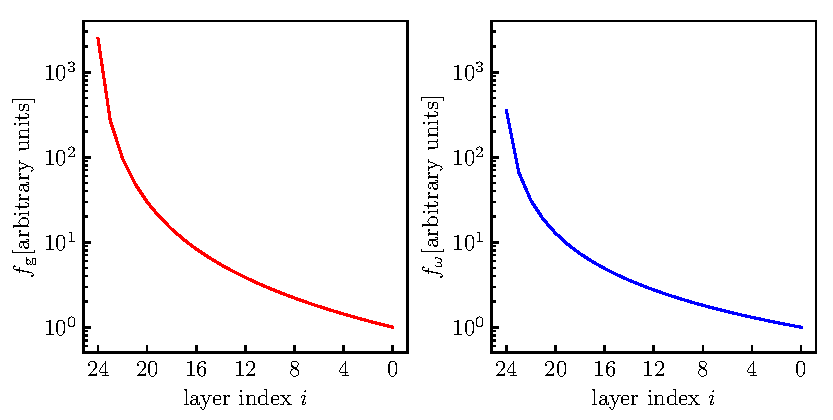
\includegraphics[width=\columnwidth]{img/plot_omega_g_profiles.pdf}
        \caption{Gravity (left) and angular velocity (right) profiles examples computed for a modeled system with radial dimension $I = 25$. The y-axis units are arbitrary because the profiles are computed relative to the outermost layer $i = 0$, where $f_{\mathrm{g} = 1}$ and $f_{\omega} = 1$.}
    \label{fig:plot_omega_g_profiles}
    \end{figure}
        
    Lastly, in our modification, $Q$ depends on the specific behavior of neighboring cells, unlike the original value defined by \eqref{eq:msm_original_odes}. Each cell essentially contains its \emph{leaky faucet}, taking the mass from other cells and redistributing it further into lower cells upon reaching the critical condition. This critical condition $z_{\mathrm{c}}$ is the same as the original MSM and is defined by \eqref{eq:z_critical_model}.

    To summarize our modification to the original MSM, the following modified ODE system server a mechanism by which the matter redistribution is triggered inside simulation cells of the MDH model

    \begin{align}
    \begin{split}
        \D{}{t} \left(m \D{z}{t}\right) &= -kz - \gamma\D{z}{t} + m f_{\mathrm{g}}, \\
        \D{m}{t} &= Q(i, j, ...),
    \end{split}
    \label{eq:msm_modified_odes}
    \end{align}

\subsection{Modeled system geometry and grid dimensions}
    Our primary focus is modeling an accretion disk of a typical \emph{cataclysmic variable star}, where the primary component would be a WD. Mass of the WD $M_{\mathrm{p}}$ can range from $0.15 M_{\odot}$ up to $1.44 M_{\odot}$, and the heaviest observed white dwarf has a mass of $1.35 M_{\odot}$ \citep{caiazzo2021}, therefore we are limited to this range when choosing primary component's mass $M_{\mathrm{p}}$.

    The inner disk radius $r_{\mathrm{in}}$ is set equal to the white dwarf's radius, which according to \citep{shapiro1983}, can be approximated by the \emph{mass to radius ratio} previously defined by \eqref{eq:mass_radius_ratio}.

    The Roche lobe of the primary component contains the outer edge of the accretion disk. Therefore the outer radius $r_{\mathrm{out}}$ is set to correspond with the binary system's Lagrange point $L_1$ and is calculated by \eqref{eq:disk_outher_radius}. Mass of the donor component $M_{\mathrm{s}}$, which also plays a role in determining the accretion disk's outer radius through its influence on Roche potential, ranges between $0.3M_{\odot}$ and $8M_{\odot}$ because the secondary star is considered to be a red-giant. 

    Having the inner and outer disk boundaries defined enables the discretization of the intermediate space into regular intervals, and the remaining parameter influencing the layer-specific radius $r_i$ is the disk's dimension $I$

    \begin{equation}
        r_i = r_{\mathrm{in}} + \frac{r_{\mathrm{out}} - r_{\mathrm{in}}}{I - 1} (I - i - 1).
    \end{equation}

    On a Keplerian orbit, the particle's orbital period, assuming there is no self-gravity interaction in the disk, is given only by the parameters $M_{\mathrm{p}}$ and $r_i$. 


    We also assume that the outermost layer of MDH shifts by exactly one \emph{angular cell length} between simulation steps. Therefore the $J$ dimension (i.e., the number of cells in one layer) and primary component's parameters provide us with the shortest producible flickering time.

    We aim to extract flickering light curves with a time scale of variability comparable to real-world observational data. Observations suggest that we need to push this time limit $\Delta t$ at least to the order minutes. To get relate the dimension $J$ and the minimal time $\Delta t$, the orbital period $\tau_{0}$ for the layer $i=0$ is needed

    \begin{equation}
        \tau_{0} = \sqrt{\frac{4 \pi^2 r_{\mathrm{out}}^3}{G M_{\mathrm{p}}}},
        \label{eq:outer_layer_tau}
    \end{equation}

    where $G$ represents the gravitational constant. So the optimal $J$ dimension is calculated

    \begin{equation}
        J = \frac{\tau_{0}}{\Delta t}.
        \label{eq:j_dimension}
    \end{equation}

    Rounding the result of \eqref{eq:j_dimension} to integer gets us the $J$ dimension for chosen minimal time $\Delta t$. Alternatively, there is a possibility of using the expression \eqref{eq:j_dimension} in reverse, starting with the chosen dimension, and the relation will give the time scale for the particular arrangement.

    The $I$ dimension is either set to a fixed chosen value or is related to the $J$ dimension. Choosing a relation that produces, at least to some degree, a spatially consistent grid of cells is advised. Throughout this study, we use the following relation, which is, again, rounded to an integer 

    \begin{equation}
        I = \frac{J}{2 \pi}.
        \label{eq:i_dimension} 
    \end{equation}

\subsection{The cellular automaton algorithm}
    The algorithm that performs the MDH simulations is a series of simple operations, including matter redistribution (i.e., the \emph{dripping} mechanism), orbital movement of its layers, and thermal processes, which are the prerequisite for light curves extraction. The algorithmic structure overview of MDH simulation is defined on the flowchart shown in figure \ref{fig:diagram_cellular_algorithm}. 

    Certain parts of the algorithm are relatively easy to parallelize, most notably the numerical solution of the ODE system \eqref{eq:msm_modified_odes}. Parallelization is almost a necessity because the number of cells for which we need to solve these equations quickly goes to thousands, even when using modest $I$ and $J$ dimensions of tens or a few hundreds of cells per dimension. Thankfully the MSM equations in individual cells are not dependent on other cells' states, so splitting the grid of solutions into multiple smaller sub-grids of tasks per step is relatively straightforward.

    \vspace*{2mm}
    
    \begin{figure}[H]
    \centering
    \begin{tikzpicture} [node distance=2cm]
        \node (start) [startstop] {Start}; 
        \node (pr1) [process, below of=start, yshift=-0.5cm] {Rotate all layers according to \eqref{eq:delta_azimuth}.}; 
        \node (pr2) [process, below of=pr1, yshift=-1cm, inner sep=0.25cm] {Find the cell closest to chosen value of $\theta$ (e.g., $\theta = 0$) in the outer layer $i = 0$, and add the $q$ amount of matter to it; see \eqref{eq:q_estimate}.}; 
        \node (pr3) [process, below of=pr2, yshift=-1.5cm] {Solve the ODE system \eqref{eq:msm_modified_odes} for all cells using an iterative method out of the Runge-Kutta family.}; 
        \node (if1) [decision, below of=pr3, yshift=-1cm] {If particular cell reaches the critical condition \eqref{eq:z_critical_model}, the mass outflow is triggered in that cell.}; 
        \node (pr4) [process, right of=if1, xshift=5.5cm] {Calculate temperature changes for all cells according to the processes described in Section \ref{sec:thermal_processes}};
        \node (pr6) [process, right of=pr2, xshift=5.5cm] {Save all cell's states.};
        \node (if2) [decision, right of=pr1, xshift=5.5cm] {End simulation?};
        \node (pr5) [process, below of=if1, yshift=-1.0cm] {Perform mass outflow of triggered cells; see \eqref{eq:delta_m}.};
        \node (stop) [startstop, right of=start, xshift=5.5cm] {Stop};

        \draw[arrow] (start) -- (pr1);
        \draw[arrow] (pr1) -- (pr2);
        \draw[arrow] (pr2) -- (pr3);
        \draw[arrow] (pr3) -- (if1);
        \draw[arrow] (if1) -- node[anchor=east] {yes} (pr5);
        \draw[arrow] (if1) -- node[anchor=south] {no} (pr4);
        \draw[arrow] (pr5) -| (pr4);
        \draw[arrow] (pr4) -- (pr6);
        \draw[arrow] (pr6) -- (if2);
        \draw[arrow] (if2) -- node[anchor=south] {no} (pr1);
        \draw[arrow] (if2) -- node[anchor=east] {yes} (stop);
    \end{tikzpicture}
        \vspace*{1mm}
    \caption{The algorithmic structure overview of MDH simulation. }
    \label{fig:diagram_cellular_algorithm}
    \end{figure}

    The discrepancy needed to be dealt with when simulation MDH is that MSM's mass scale is different from the global (i.e., real-world) mass scale of the accretion disk. However, it is not a big problem. MSM is used only as the critical condition because of its qualitative and not quantitative properties. Nevertheless, we need to know the \emph{real} amount of accreted matter. For a typical CV, the accretion rate is assumed \citep{ae_shortrev2015}

    \begin{equation}
        \dot{M} \sim 10^{14}\, \mathrm{g \cdot s^{-1}},
    \end{equation}

    and the value of $a$ according to \citep{msmm1999} is

    \begin{equation}
        \label{eq:q_estimate}
        q \sim 10^{-1}\, \mathrm{g},
    \end{equation} 

    so, we can easilly relate the \emph{real} accretion rate $\dot{M}$ to the internaly defined $q$

    \begin{equation}
        q \propto \dot{M} \cdot \Delta t.
    \end{equation}

    The mass addition to the outer layer $i = 0$ that models the matter accretion through the Lagrange point $L_1$ would fill up only the outer layer. Therefore the subsequent layers are filled from the adjacent cells \emph{above} when they reach the critical condition \eqref{eq:z_critical_model}.

    Part of the mass is separated from the source cell as the moment of \emph{dripping} and transfers into lower cells. The amount of mass $\Delta m$ that breaks is

    \begin{equation}
        \Delta m = \psi \cdot m_{ij}
        \label{eq:delta_m}
    \end{equation}

    where the value of $\psi \in [0;1]$ is the drop breakout ratio, which serves as another free parameter of the simulation. The numerical stability of the simulation is ensured by introducing a low-value cut-off for the cell's mass $m_{ij}$. The following formula is used to compute the cell's remaining mass after the breakout    

    \begin{equation}
        \begin{aligned}
            & m_{ij}~= 
            \begin{cases}
                m_{ij} - \Delta m \hspace{5mm} (m_{ij} \ge 10^{-8}) \\
                \hspace{8mm} 0 \hspace{12.5mm} (m_{ij} < 10^{-8}).
            \end{cases}
        \end{aligned}
        \label{eq:m_cut_off}
    \end{equation}

    There are always no more than two lower layer cells in contact with the source cell, as evident from Figure~\ref{fig:grid_states}. Therefore, the redistribution algorithm finds the two closest cells and splits the mass $\Delta m$ between the two receiving cells. The mass split is directly proportional to the relative length of contact the adjacent cells have with the source cell.

% -----------------
% Thermal processes  
% -----------------
\section{Thermal processes}
\label{sec:thermal_processes}
    The crucial quantity for our model's evaluation is the extracted synthetic light curve, which we derive from the disk's radiation properties, primarily the temperature. The temperature must be known for all cells at any moment of the simulation. We assume that the cells exhibit black-body radiation and are optically thin. 

    The cell temperature continuously changes and depends on the previous states rather than being a function of only current internal and external parameters. Because of the matter redistribution processes (i.e., the dripping and rotational mixing), the temperature changes are carried throughout the disk's body. The starting point of this chain of changes is matter inflow in the outer layer $i = 0$. The given parameters of the donor star determine the inflow temperature. For the late-type star, according to \citep{allen1973}, it is estimated

    \begin{equation}
    T_{\mathrm{out}} \sim 10^3\, \mathrm{K}.
    \end{equation}

    We identified three processes influencing the cell's temperature. In the following sections, we will describe those in detail and get the final cell's temperature as their summary. 

\subsection{Free-Free emission heating}
    The matter that beaks out by \emph{dripping} losses a part of its potential energy, which, according to \citep{yonehara1997}, is calculated by 

    \begin{equation}
    \Delta E_{ij} = \frac{1}{2} G M_{\mathrm{p}} \Delta r \frac{\Delta m_{ij}}{r_i^2},
    \label{eq:e_pot}
    \end{equation}

    where the amount of falling mass is represented by $\Delta m_{ij}$ and $\Delta r$ is the layer width (i.e., the distance traveled by the mass). This energy is released by the process of \emph{free-free emission} (i.e. bremsstrahlung); with some efficiency $\varepsilon$ is transformed into internal energy $U$ of the receiving cell

    \begin{equation}
        \Delta U_{i+1,j} = \varepsilon \Delta E_{ij},
    \end{equation}

    where $\Delta U_{i+1,j}$ represents the change of receiving cell's internal energy that heats the cell. For the sake of simplicity, we consider the heating efficiency to be ${\varepsilon=1}$, then  

    \begin{equation}
        \Delta U_{i+1,j} \equiv \Delta E_{ij}.
        \label{eq:e_int_pot_equiv}
    \end{equation} 

    Internal energy changes in relation to the temperature according to 

    \begin{equation}
        \Delta U_{ij} = \frac{3}{2} n_{ij} \mathcal{R} \Delta T_{ij},
        \label{eq:e_int_temp_relation}
    \end{equation}

    where $\mathcal{R}$ represents the ideal gas constant, and $n_{ij}$ is the number of gas moles in the cell. We assume the gas mostly consists of hydrogen, whose molar mass is $M_{\mathrm{H}} \approx 1$; therefore, the mass $m_{ij}$ and the number of moles $n_{ij}$ are interchangeable. Substitution of \eqref{eq:e_int_temp_relation} and \eqref{eq:e_pot} into \eqref{eq:e_int_pot_equiv}, and a bit of rearrangement, yields the relation of cell's temperature change in layer $i+1$, and the amount of mass falling from the donor cell

    \begin{equation}
        \Delta T_{i+1,j} = \frac{1}{3} \frac{G M_{\mathrm{p}} \Delta m_{ij} \Delta r}{r_{i}^2 \mathcal{R} m_{i+1,j}}.
        \label{eq:temp_ff_final}
    \end{equation}

\subsection{Gas mixing}
    The second mechanism concerns mixing different temperatures and amounts of gases when dripping happens. We need to describe the donor cell's temperature change $T_{ij}$ and the receiving cell's $T_{i+1,j}$. We get both by utilizing changes in the cell's internal energy. The resulting expression for the donor cells is simply  

    \begin{equation}
    T_{ij}' = T_{ij},
    \end{equation}

    where $T_{ij}$ and $T_{ij}'$ are the temperatures before and after the mass outflow, respectively. The mixing of two different amounts of gas at two different temperatures is happening on the receiving cell's side. The expression for the receiving cell is

    \begin{equation}
    T_{i+1,j}' = \frac{m_{i+1,j} T_{i+1,j} + \Delta m_{ij} T_{ij}}{m_{i+1,j} + \Delta m_{ij}}.
    \end{equation}

\subsection{Radiative cooling}
    The last mechanism taking part in the cell's temperature changes is radiative cooling. The cell's radiation of optically thin disk is approximated as black-body radiation that emits through the top and bottom facets of each cell, and one facet having the area

    \begin{equation}
        S_{ij} = \frac{2 \pi r_i \Delta r}{J},
        \label{eq:facet_area}
    \end{equation}

    where the layer width is represented by $\Delta r$. Therefore cell's internal energy conversion to its black-body radiation is

    \begin{equation}
        \frac{3}{2} m_{ij} \mathcal{R} \frac{dT_{ij}}{dt} = \sigma T_{ij}^4 S_{ij},
        \label{eq:rad_cooling_temp_0}
    \end{equation}

    where $\sigma$ is the Stefan-Boltzman constant. Integration of \eqref{eq:rad_cooling_temp_0} and yields the expression for the cell's temperature, which is in the local thermodynamic equilibrium of the radiative cooling

    \begin{equation}
    T_{ij}' = \left( \frac{2 \sigma S_{ij} t}{m_{ij} \mathcal{R}} + \frac{1}{T_{ij}^3} \right)^{-1/3}.
    \end{equation}

% --------------------------------
% Synthetic light curve extraction
% --------------------------------
\section{Synthetic light curves}
    Synthetic light curve extraction starts with the full knowledge of temperatures throughout the simulation as a product of previously defined thermal processes. This information enables us to extract simulated spectra from the disk's radiation. Wavelength-specific radiation power of individual cells is given by

    \begin{equation}
        L_{\lambda,ij} = 4\pi \cdot S_{ij} \cdot B_{\lambda,ij}(\lambda, T_{ij}),
        \label{eq:facet_radiation}
    \end{equation}

    where $B_{\lambda}(\lambda, T_{i,j})$ represents flux density in the given point by Planck's function. Single radiating facet area $S_{ij}$ is defined by \eqref{eq:facet_area}, and the accretion disk, considered optically thin, radiates through a single face into the solid angle of $2\pi$. 

\subsection{Light curves in a photometric filter}
    To achieve a closer observational data analogy, we use analytic approximations of Johnson-Cousins $\mathcal{UBVRI}$ filters that are applied to the wavelength-specific total power output of the disk. This filtering process produces the synthetic light curve as it would be observed through the chosen filter. The approximation is expressed by

    \begin{equation}
    g(\lambda) \propto \mathrm{exp}\left[ - \frac{1}{2} \left( \frac{\lambda - \lambda_{\mathrm{c}}}{\lambda_{\mathrm{w}}} \right)^2 \right],
    \label{eq:filter_gauss}
    \end{equation}

    where filter-specifig effective central wavelength is $\lambda_{\mathrm{c}}$, and $\lambda_{\mathrm{w}}$ sets the effective filter width. Johnson-Cousins approximative values are listed in Table \ref{tab:johnson_cousins_approx}.

    \begin{table}[ht]
    \centering
    \begin{tabular*}{\columnwidth}{@{\extracolsep{\fill}}ccc}
    Filter & $\lambda_{\mathrm{c}}$ $[\mathrm{\r{A}}]$ & $ \lambda_{\mathrm{w}}$ $[\mathrm{\r{A}}]$\\
    \hline\hline
    $\mathcal{U}$ & 3663 & 650\\
    $\mathcal{B}$ & 4361 & 890\\
    $\mathcal{V}$ & 5448 & 840\\
    $\mathcal{R}$ & 6407 & 1580\\
    $\mathcal{I}$ & 7980 & 1540\\
    \hline
    \end{tabular*}
    \caption{Parameters of Johnson-Cousins $\mathcal{UBVRI}$ filters approximation. \citep{bessell2005}}
    \label{tab:johnson_cousins_approx}
    \end{table}

    We calculate every cell's radiation power step by step. Using \eqref{eq:facet_radiation} and \eqref{eq:filter_gauss} and summing up all the cells, we get filtered power output $L_{\mathrm{F}}$ from both accretion disk's sides

    \begin{equation}
    L_{\mathrm{F}} = 4 \pi S_{ij} \Delta \lambda \sum_{i=0}^{I-1} \sum_{j=0}^{J-1} \sum_{\lambda=0}^{\infty} B_{\lambda,ij}(\lambda, T_{ij})\,g(\lambda),
    \end{equation}

    where $\Delta \lambda$ is the wavelength integration step.

    
    % 7. MODEL IMPLEMENTATION 
    %&<latex>
\chapter{MDH - MODEL IMPLEMENTATION}
\label{chap:model_implementation}
\thispagestyle{empty}
\mquote{Computer science is no more about computers than astronomy is about telescopes.}{Edsger Dijkstra}

    This chapter will focus on the technical side of our accretion disk modeling efforts. Because incomparably more time was spent on implementing, testing, and debugging the code than developing the underlying theory; we are talking orders of magnitude more.

    There were four consecutive versions of the code. Each is improving the previous and fixing its errors while introducing new challenges. The version presented in this study is the last iteration so far, and as with any other software, whether the scientific or commercial application, it is never finished. There is still room for improvement and new ideas. However, we can confidently say that this version of MDH implementation can model accretion disc dynamics and power output with a good mix of robustness and customizability.  

    We knew from the start that modeling such a complex, inherently non-linear system would be a challenge, first and foremost hardware-wise. Because for one, as shown in Chapter \ref{chap:multilayer_dripping_handrail}, the number of individual cells, each holding its system of ODEs, can quickly go up to thousands. Second, each cell holds 13 state values (i.e., coordinates, temperature, compute flags, etc.). For example, a moderate simulation run of $10^5$ steps produces over a $100 \si{\giga\byte}$ of data, and that is just the dynamical simulation part. When we start radiation extraction out of these results, we face several $\si{\tera\byte}$ datasets because, for every cell, we need to compute a spectral energy distribution of a few hundred values (depending on the chosen range and granularity). Therefore, two challenges were presented from the get-go:

    \begin{enumerate}
        \item[\textbf{a)}] Solving a large number of ODE sets.
        \item[\textbf{b)}] Handling a large amount of data. 
    \end{enumerate}

    While \textbf{a)} is achievable to some degree by parallelization and good optimization, the \textbf{b)} is just a matter of having enough data storage; there is no way around it. Ultimately, we created a simulation code that is usable even on computer systems with relatively modest hardware specifications. For reference, simulation examples presented in this study were done on a personal desktop computer with Intel's Core i7-4790k CPU, 32$\si{\giga\byte}$ of memory, and large enough storage to accommodate the simulation data output. With this configuration, every presented simulation took several hours at most. 

    MDH is implemented as purely CLI (\emph{Command Line Interface}) application because there is no need for GUI (\emph{Graphical User Interface}). It runs under the Linux operating system (currently tested with kernel versions 5.0 and higher). A detailed description of command line arguments can be found in the documentation available at \url{https://github.com/Preqsis/multilayer-dripping-handrail}

\section{Algorythmic overview}
    All the core simulation code is implemented in \CC. There are also supporting scripts for visualization, input preparation, data sorting, and extraction written in Python 3.9+.  

\subsection{Model's subtasks}
    The model's codebase is split, based on the logic of consequent operations, into three parts that, for the sake of simplicity and ease of use are:

    \begin{enumerate}[topsep=4mm]
        \item \textbf{SIMULATION} (SIM) - performs the dynamical simulation of matter flow and temperature changes in the accretion disc.
        \item \textbf{RADIATION} (RAD) - takes the dynamical simulation results and computes the disc's power output spectral distribution over the predefined range of wavelengths.
        \item \textbf{OBSERVATION} (OBS) - performs a synthetic observation, with the use of analytical approximations of Johnson-Cousins $\mathrm{UBVRI}$ photometric filters, and extracts a flickering light curve.  
    \end{enumerate}

    All these subtasks employ parallelization, but each in a slightly different fashion. SIM and RAD are parallelized spatially, which means that the disc's cells are split into same-sized groups, and these groups are computed separately by individual processes. OBS is parallelized in the time domain because the computation of an individual light curve's data point is not dependent on previous or following data points. 

    The subtasks can be run separately or pass over its result to the next subtask. Also, in the case of SIM, it is possible to run it either as a clean simulation or as a continuation of previous results. The ability to start the SIM from a predefined point in another run is particularly important in cases where we need to simulate multiple parameter variations with the same initial conditions. It might seem easy, but re-initializing such a complex and large data structure is not trivial. 

\subsection{Open MPI paralelization}
    Open MPI (Message Passing Interface) is an open-source, high-performance message-passing library that serves as a communication protocol in distributed parallel computing \citep{openmpi2022}. It is widely used, but not limited to, by many supercomputers. In addition, its ease of use, good documentation, and large community of developers make it relatively straightforward, even on smaller projects like ours. 

    We use a simple approach of running one \mbox{MASTER} process and multiple SLAVE processes. The \mbox{MASTER} is the primary handler of the distributed computation that sends instructions to the SLAVES and then collects, sorts, and outputs the results. The SLAVE performs most of the computations based on the data and instructions received from the \mbox{MASTER}, for example, a subset of MDH cells. For reference, for the results presented in this study, that usually means one \mbox{MASTER} plus seven SLAVES.

    One downside, or rather a complication when using MPI, is that the data types need to be explicitly defined and precisely allocated because each end of MPI communication expects the same predefined data type with uniform memory allocation. For MDH implementation, it means, in some cases, a four-dimensional array of pointers.

\subsection{\mbox{MASTER} processes}
    The algorithm of the \mbox{MASTER} process is very similar for all three MDH subtasks, there are slight differences, but the set of operations and their order is the same. The generalized overview of the \mbox{MASTER} process's algorithm is shown in Figure~\ref{fig:diagram_master_process}.  

    \begin{figure}[H]
    \begin{center}
    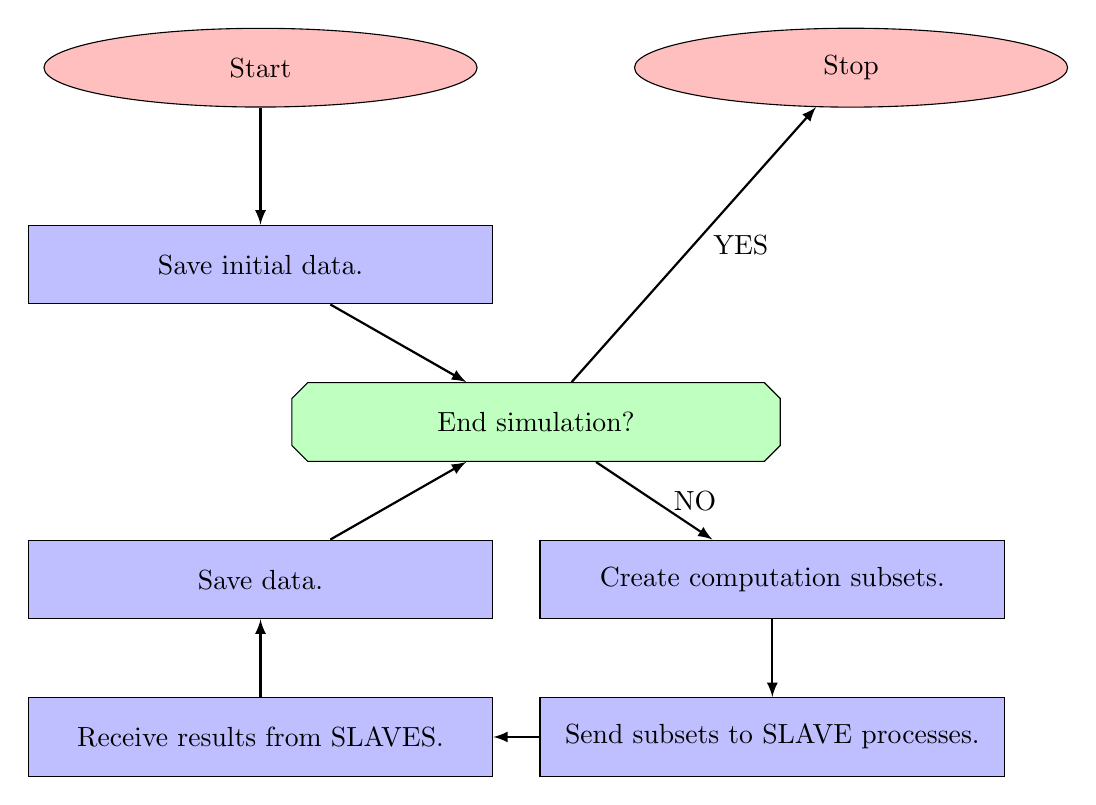
\begin{tikzpicture} [node distance=2cm]
        \node (start) [startstop] {Start}; 
        \node (stop) [startstop, right of=start, xshift=5.5cm] {Stop};
        \node (pr1) [process, below of=start, yshift=-0.5cm] {Save initial data.};
        \node (if1) [decision, below of=pr1, xshift=3.5cm] {End simulation?};
        \node (pr2) [process, below of=if1, xshift=3cm] {Create computation subsets.};
        \node (pr3) [process, below of=pr2] {Send subsets to SLAVE processes.};
        \node (pr4) [process, left of=pr3, xshift=-4.5cm] {Receive results from SLAVES.};
        \node (pr5) [process, left of=pr2, xshift=-4.5cm] {Save data.};

        \draw[arrow] (start) -- (pr1);
        \draw[arrow] (pr1) -- (if1);
        \draw[arrow] (if1) -- node[anchor=west] {\ YES} (stop);
        \draw[arrow] (if1) --  node[anchor=west] {\ NO} (pr2);
        \draw[arrow] (pr2) -- (pr3);
        \draw[arrow] (pr3) -- (pr4);
        \draw[arrow] (pr4) -- (pr5);
        \draw[arrow] (pr5) -- (if1);
    \end{tikzpicture}
    \end{center}
    \vspace{6mm}
    \caption{Overview of the generalized \mbox{MASTER} process's algorithm.}
    \label{fig:diagram_master_process}
    \end{figure}

\subsection{SLAVE processes}
    The \mbox{SLAVE} process structure also follows the same basic order of operations for all three MDH subtasks, differing mainly in the performed computations. A generalized overview of the SLAVE process's algorithm is shown in Figure~\ref{fig:diagram_slave_process}.

    \begin{figure}[H]
    \centering
    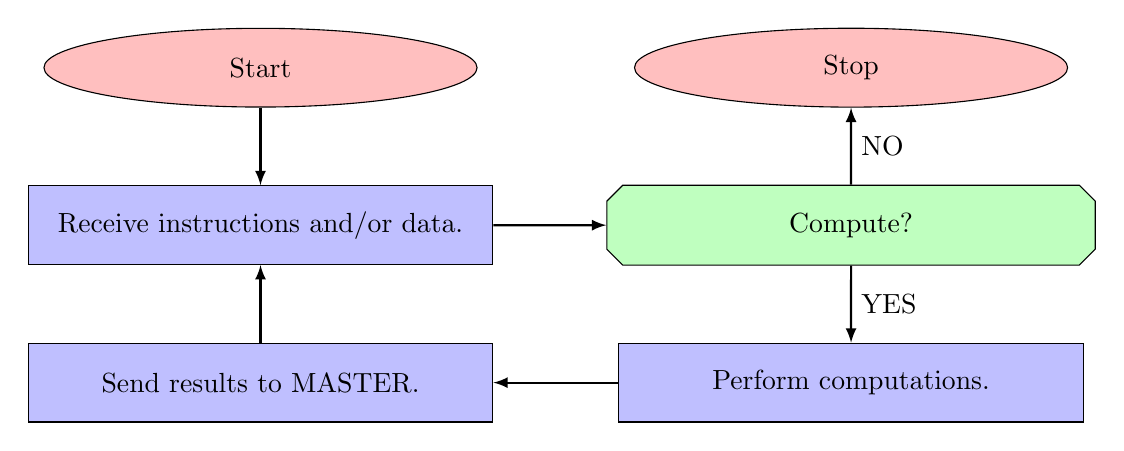
\begin{tikzpicture} [node distance=2cm]
        \node (start) [startstop] {Start}; 
        \node (stop) [startstop, right of=start, xshift=5.5cm] {Stop};
        \node (pr1) [process, below of=start] {Receive instructions and/or data.};
        \node (if1) [decision, right of=pr1, xshift=5.5cm] {Compute?};
        \node (pr2) [process, below of=if1] {Perform computations.}; 
        \node (pr3) [process, left of=pr2, xshift=-5.5cm] {Send results to \mbox{MASTER}.};

        \draw[arrow] (start) -- (pr1);
        \draw[arrow] (pr1) -- (if1);
        \draw[arrow] (if1) -- node[anchor=west] {NO} (stop);
        \draw[arrow] (if1) -- node[anchor=west] {YES} (pr2);
        \draw[arrow] (pr2) -- (pr3);
        \draw[arrow] (pr3) -- (pr1);
    \end{tikzpicture}
    \vspace{6mm}
    \caption{Overview of the generalized SLAVE process's algorithm.}
    \label{fig:diagram_slave_process}
    \end{figure}

\subsection{Data output}
    To store a large amount of data that MDH simulation produces, we use HDF5 (\emph{Hierarchical Data Formats}), which is an open-source file format that can store complex and heterogeneous data \citep{hdf5_2006}. Furthermore, HDF5 supports very fast IO (\emph{Input/Output}), so it enables us to store every simulation frame (i.e., the state in time) in full without the need for data truncation or frame skipping. At the same time, the simulation performance, at least with our example hardware configuration, is not limited by the IO but only by the CPU. 

    Every data frame, whether SIM, RAD, or OBS data, is stored as a multidimensional array with the same structure used in computations, making re-initializing the simulation run easier. HDF5 also can store meta-data, which means we can also store the global simulation parameters (e.g., disc's geometry, central object's mass, size of the timestep, etc.) alongside the actual data; therefore, the whole simulation is reproducible with just one file, without the need for additional meta-data or configuration files.

    HDF5 was an excellent fit for our model's needs because it solved significant IO limitations in the first version of MDH.

\subsection{ODE solver}
    We use a numerical integrator out of the Runge-Kutta family to solve the MSM's ODE system. By default, it uses Fehlberg's seventh and eighth-order method, which is implemented by the boost::numeric::odeint module \citep{boost_2007}. The selected stepper method can be changed using the dedicated CLI parameter of the MDH application. 

\section{SIM - dynamical simulation subtask}
    The SIMULATION subtask is the starting point of the model's computational pipeline and the algorithmically most complex part of the code. It performs the dynamical matter redistribution simulation based on predefined MDH rules and geometry (see. Chapter \ref{chap:multilayer_dripping_handrail}). Solving the MSM ODE system is essential because it is the crucial mechanism triggering the matter accretion to lower layers. This subtask is spatially parallelized and uses the \mbox{MASTER/SLAVE} process paradigm.

    The \mbox{MASTER} process of SIM subtasks performs the data handling and instruction distribution role. First, it splits the accretion disk into $n-1$ cell subsets, where $n$ is the total number of running MDH processes, and then the subsets are distributed into the running SLAVE processes.

    When the SLAVE processes are done with their calculations, the \mbox{MASTER} collects and combines the results. Also, the check for MSM critical dripping conditions must be done in \mbox{MASTER} because the matter redistribution happens all over the disc's body, across and between all the subsets of cells. Lastly, it saves the completed frame results into the HDF5 (*.h5) data file. 

    The SLAVE processes of SIM are the actual \emph{simulation} part of this subtask. They receive the cell subsets, carry out the MSM's ODE system solution over those subsets, and return the results to \mbox{MASTER}. 

    This back-and-forth communication between the processes and data saving is repeated step by step for the whole simulation run. 

\subsection{Disturbing the simulation by matter outburts}
    \label{sec:distributed_sim}
    We implemented a possibility to disturb the MDH's SIM computation by a sudden targeted matter addition, which is supposed to model the situation when a matter outburst from the system's secondary component falls onto the accretion disc's body. 

    The disturbance is done by supplying a *.json blob definition file, which defines the position, size, and timing for the matter addition to the disc. We generally use a spherical blob of predefined total mass and gradually increasing density towards its center. The blob is divided into slices that are deposited onto the disc.

\section{RAD - radiation extraction subtask}
    The RADIATION subtask takes the results of the SIMULATION subtask, and per-cell basis computes the spectral energy distribution on a predefined wavelength interval, using \emph{black-body approximation} for disc's cells. This subtask is also spatially parallelized and employs the \mbox{MASTER} and SLAVES process model.

    The structure and order of operations are the same as for SIM. However, the RAD's SLAVE processes compute the spectral energy distribution for each cell, which means a lot more values per single cell than SIM; therefore, the HDF5 output is drastically bigger. For reference, the RAD results from which we extracted the light curves in Chapter \ref{chap:cv_models} are done for the interval of $2880$ steps (i.e., $48$ hours in the real world), and the single RAD HDF5 data file is over 600 $\si{\giga\byte}$.

\section{OBS - synthetic observation subtask}
    Third and last in the MDH computation pipeline is the OBSERVATION subtask, which serves as a synthetic light curve extractor. It takes the results of RAD and applies analytical approximations of Johnson-Cousins $\mathcal{UBVRI}$ photometric filters. This subtask is also parallelized similarly to RAD and OBS and uses the same \mbox{MASTER}/SLAVE approach, but in this case, the data subsets are defined in the time domain. 

    It is almost ironic that the output of OBS is only a few hunderd $\si{\kilo\byte}$ HDF5 data file, considering the input is the RAD data file, which is the multi-hunderd $\si{\giga\byte}$ behemoth. The reason is that the output data are just a few simple time series of several thousand steps for each Johnson-Cousins photometric filter approximation (i.e., the light curves).

\section{Results visualization}
% TODO: dopsat sekci o vizualizaci s priklady



    
    % 8. CV - MODEL
    %&<latex>
\chapter{CV MODELS}
\label{chap:cv_models}
\thispagestyle{empty}

\mquote{640K ought to be enough for anybody}{Bill Gattes}
    In this Chapter, we will present several examples of MDH results. The MDH has two free parameters to alter the outcome of SIM: 

    \begin{enumerate}
        \item The local MSM inflow $q \sim 10^{-1}$.
        \item The drop breakout ratio $\psi \in \langle 0; 1 \rangle$.
    \end{enumerate}

    The $q$ controls the relationship between real-world accretion disk mass inflow $Q$ and MSM's development toward drop breakout. The lower value of $q$ means that it takes longer for the MSM ODE system to reach its critical condition, therefore, how often the individual cells drip. The breakout ratio $\psi$ controls the amount of mass that breaks out from the cell at the moment of dripping. Both of these parameters control the mass flow rate in the disc's body and could be considered a viscosity model of the accreted medium. 

    As a demonstration, we ran simulations with multiple $q$ and $\psi$ variations with relatively high and low values for both parameters. Furthermore, we conducted undisturbed and disturbed SIM for each specific combination of parameters. By disturbed, we mean a dynamical flow simulation with a sudden mass outburst from the secondary component (see Section \ref{sec:distributed_sim}).

    All SIM runs used the same CV system parameters

    \begin{align}
    \begin{split}
        M_{\mathrm{p}} &= 0.63 M_{\odot}, \\
        r_{\mathrm{in}} &= 0.01 R_{\odot}, \\
        r_{\mathrm{out}} &= 1.16 R_{\odot}, \\
        \dot{M} &= 10^{14} \si{\gram \cdot \second^{-1}}, \\
        T_{\mathrm{out}} &= 4500 \si{\kelvin},
    \end{split}
    \end{align}

    where $M_{\mathrm{p}}$ represents the mass of the CV's primary component (i.e., the white dwarf). Radii $r_{\mathrm{in}}$ and $r_{\mathrm{out}}$ correspond to the inner and outer edge of the accretion disk, respectively. The accretion rate is represented by $\dot{M}$, and the initial temperature of the accreted matter is $T_{\mathrm{out}}$.

\section{Undisturbed SIM}
    We choose four combinations of $q$ and $\psi$ to conduct the SIM runs. Table \ref{tab:table_simultation_cases_undisturbed} lists the specific details of each SIM run.

    \begin{table}[ht]
    \centering
    \begin{tabular*}{\columnwidth}{@{\extracolsep{\fill}}cccccc}
    SIM run & $q$ & $\psi$ & $n [\mathrm{steps}]$ & $I$ & $J$ \\ 
    \hline\hline
        C1 & $0.1$ & $0.1$ & $2880$ & $42$ & $265$ \\
        C2 & $0.1$ & $0.9$ & $2880$ & $42$ & $265$ \\
        C3 & $0.9$ & $0.1$ & $2880$ & $42$ & $265$ \\
        C4 & $0.9$ & $0.9$ & $2880$ & $42$ & $265$ \\
    \hline
    \end{tabular*}
    \caption{Undisturbed SIM runs parameter variations.}
    \label{tab:table_simultation_cases_undisturbed}
    \end{table}

    We designate the individual SIM runs as C1 through C4 for easier orientation. All runs are done using the same grid dimensions $I$ and $J$, for the same time duration of $2880$ simulation steps and are started after the initial filling state of $2 \cdot 10^5$ steps. 

\subsection{C1 - unstable filling stage}
    In this case, when both $q$ and $\psi$ are set to be relatively low values (i.e., very viscous medium), the MDH does not produce a stable accretion disc. Instead, there is a limiting inner radius of the stable accretion flow, and unstable matter outbursts fill the inner regions through individual cells on the inner edge of the stable accretion ring. 
    Figure~\ref{fig:plot_density_temperature_c1} show the occurrence of such outburst at approximately $7 \cdot 10^4$ steps into the initial filling SIM run, where on the left, we see the area density distribution and on the right, the corresponding temperature of individual cells.

    Due to its instability, the C1 SIM run is omitted from the synthetic observations. However, it would undoubtedly require more investigation into this high-viscosity case.  

\subsection{C2 - gradual density increase and uniform temperature}
    C2 SIM run demonstrates the case when the MSM's flow parameter $q = 0.1$ is set relatively low, and the breakout ratio $\psi = 0.9$ is set relatively high. Figure~\ref{fig:plot_density_temperature_c2} shows that this combination produces a gradual increase in area density towards the center of the disc and uniform temperature distribution with typical values from $T \sim 10^2 \si{\kelvin}$ to $T \sim 10^3 \si{\kelvin}$. 

    This outcome could be explained by the higher value of $\psi$ moving the matter inward more quickly by breaking out larger parts of matter by dripping. At the same, the low value of $q$ means that the total amount of accreted matter is relatively low; therefore, its cooling rate is higher when it loses energy during the fall inward. 

\subsection{C3 - density bump and temperature waves}
    C3 SIM run is particularly interesting because the bump in the area density close to the center of the accretion disc but not at the very inner edge is especially pronounced. However, this feature is present in other SIM run results too. Also, the temperatures throughout the disc are considerably higher than C2, with values ranging from $T \sim 10^3\si{\kelvin}$ to $T \sim 10^4\si{\kelvin}$. C3 results are shown in Figure~\ref{fig:plot_density_temperature_c3}. 

    An interesting feature of C3 is the temperature waves visible in the temperature distribution plot. Furthermore, there are highly localized temperature spikes several orders of magnitudes higher than the surrounding matter.

\subsection{C4 - density spikes and colder inner regions}
    C4 SIM run shown in Figure~\ref{fig:plot_density_temperature_c4} produce mostly uniform area density distribution with localized increases grouped around a relatively narrow range of radii. The temperature distribution exhibits higher temperatures closer to the accretion disc's edge, while the inner regions are about one order of magnitude colder. 

    The low, uniform area density and the higher temperatures on the outer edge could be explained by high values of both $q = 0.9$ and $\psi = 0.9$ (i.e., low viscosity medium) because the MSM ODE system reaches the critical condition relatively quickly. The high breakout ratio $\psi$ ensures that a large portion of cells' content is carried away by dripping. Therefore at the edge, the temperature could be a product of slow radiative cooling of the medium at the original inflow temperature carried in from the secondary star. The high matter flow enables rapid cooling and produces a temperature decrease in the inner regions.

\section{Disturbed simulations}
    For the SIM runs disturbed by the blob impacts, we used the same initial conditions and parameter variations as for the undisturbed runs. Table~\ref{tab:table_simultation_cases_disturbed} lists the used parameter settings.

    \begin{table}[ht]
    \centering
    \begin{tabular*}{\columnwidth}{@{\extracolsep{\fill}}cccccc}
        SIM run & $q$ & $\psi$ & $n [\mathrm{steps}]$ & $I$ & $J$ \\ 
    \hline\hline
        C5 & $0.1$ & $0.9$ & $2880$ & $42$ & $265$ \\
        C6 & $0.9$ & $0.1$ & $2880$ & $42$ & $265$ \\
        C7 & $0.9$ & $0.9$ & $2880$ & $42$ & $265$ \\
    \hline
    \end{tabular*}
    \caption{}
    \label{tab:table_simultation_cases_disturbed}
    \end{table}

    The SIM run C5 uses the same initial condition as C2, C6 as C3, and C7 initial conditions are equivalent to C4. The blobs' size, shape, and timing were identical between all three runs. There were three blob impacts per run in short succession of similar sizes $M_{\mathrm{blob}}\sim 10^{17} \si{\gram}$. Figures~\ref{fig:plot_density_temperature_c5},~\ref{fig:plot_density_temperature_c6},~and~\ref{fig:plot_density_temperature_c7} show the C5, C6 and C7 results, respectivelly.

    It is most apparent from C5 and C7 that the blob impacts induce localized high-temperature spikes along the path of newly added matter. At the same time, the blob matter increases the disc's temperature due to the higher temperature carried in from the secondary star. Figures~\ref{fig:plot_density_temperature_c5}~through~\ref{fig:plot_density_temperature_c7} all depict the exact moment in their respective SIM runs.

\section{Synthetic light curves}
    We also computed the synthetic light curves for all simulation cases C2 through C7. Figures~\ref{fig:plot_light_curves_undisturbed}~and~\ref{fig:plot_light_curves_disturbed} demonstrate that, depending on the chosen combination of free parameters, we get vastly different light curves. 

    The undisturbed cases are shown in Figure~\ref{fig:plot_light_curves_undisturbed}. For the C2 SIM run, we see relatively low power output with very short brightness spikes. The C3 light curve exhibits active aperiodic flickering, while the C4 shows periodic longer-lasting increases in power output. 

    Similarly, for the disturbed cases C5, C6, and C7, we see that the high value of $\psi = 0.9$ produces a significantly shorter stage of increased brightness due to the blob impacts (see Figure~\ref{fig:plot_light_curves_disturbed} a) and c)) because the high breakout ratio speeds up the mass accretion. 

    \begin{sidewaysfigure}[h]
        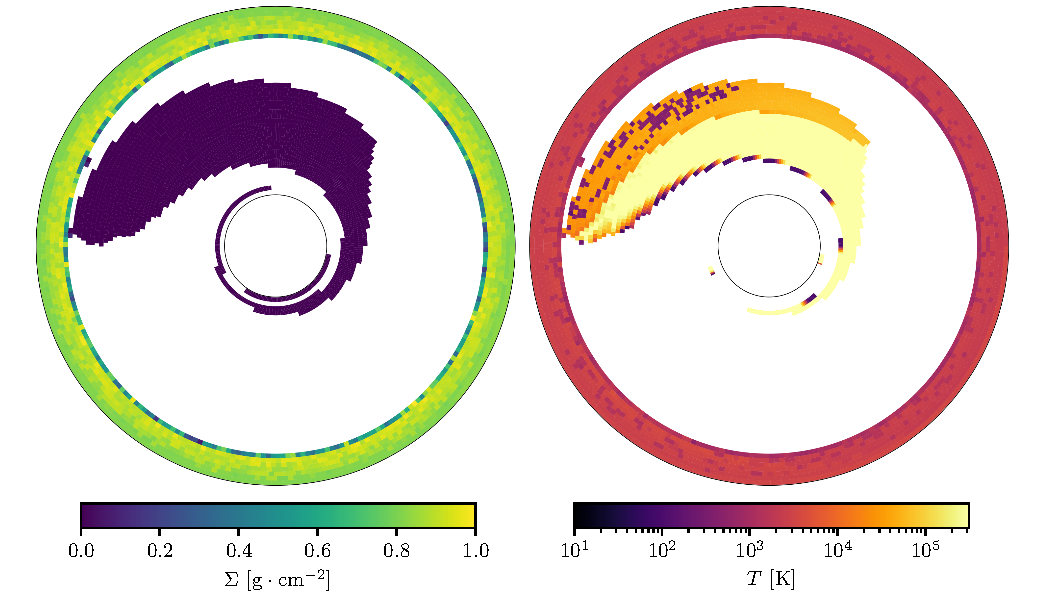
\includegraphics[width=1.0\columnwidth]{img/plot_density_temperature_c1.pdf}
        \caption{C1 ($q = 0.1$, $\psi = 0.1$) - Snapshot of the outburst from the outer stable accretion region at $7 \cdot 10^4$ steps into the SIM run.}
        \label{fig:plot_density_temperature_c1}
    \end{sidewaysfigure}

    \begin{sidewaysfigure}[h]
        \includegraphics[width=1.0\columnwidth]{img/plot_density_temperature_c2.pdf}
        \caption{C2 ($q = 0.1$, $\psi = 0.9$) - Arbitrary step in the SIM run of 2880 steps.}
        \label{fig:plot_density_temperature_c2}
    \end{sidewaysfigure}

    \begin{sidewaysfigure}[h]
        \includegraphics[width=1.0\columnwidth]{img/plot_density_temperature_c3.pdf}
        \caption{C3 ($q = 0.9$, $\psi = 0.1$) - Arbitrary step in the SIM run of 2880 steps.}
        \label{fig:plot_density_temperature_c3}
    \end{sidewaysfigure}

    \begin{sidewaysfigure}[h]
        \includegraphics[width=1.0\columnwidth]{img/plot_density_temperature_c4.pdf}
        \caption{C4 ($q = 0.9$, $\psi = 0.9$) - Arbitrary step in the SIM run of 2880 steps.}
        \label{fig:plot_density_temperature_c4}
    \end{sidewaysfigure}
    
    \begin{sidewaysfigure}[h]
        \includegraphics[width=1.0\columnwidth]{img/plot_density_temperature_c5.pdf}
        \caption{C5 ($q = 0.1$, $\psi = 0.9$) - Snapshot shortly after the blob impact in the disturbed SIM run of 2880 steps.}
        \label{fig:plot_density_temperature_c5}
    \end{sidewaysfigure}

    \begin{sidewaysfigure}[h]
        \includegraphics[width=1.0\columnwidth]{img/plot_density_temperature_c6.pdf}
        \caption{C6 ($q = 0.9$, $\psi = 0.1$) - Snapshot shortly after the blob impact in the disturbed SIM run of 2880 steps.}
        \label{fig:plot_density_temperature_c6}
    \end{sidewaysfigure}

    \begin{sidewaysfigure}[h]
        \includegraphics[width=1.0\columnwidth]{img/plot_density_temperature_c7.pdf}
        \caption{C7 ($q = 0.9$, $\psi = 0.9$) - Snapshot shortly after the blob impact in the disturbed SIM run of 2880 steps.}
        \label{fig:plot_density_temperature_c7}
    \end{sidewaysfigure}
    
    \begin{figure}
    \begin{center}
        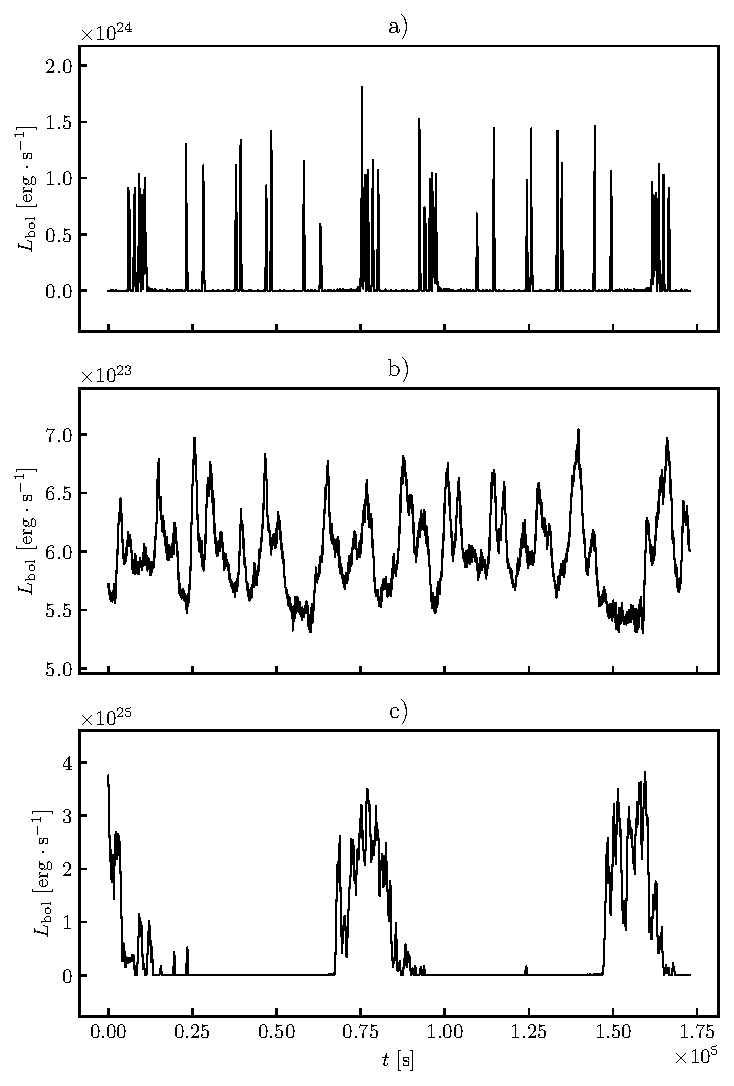
\includegraphics[width=1.0\textwidth]{img/plot_light_curves_undisturbed.pdf}
    \end{center}
    \caption{Synthetic light curves extracted from the undisturbed SIM runs: \mbox{a) C2 ($q = 0.1$; $\psi = 0.9$), b) C3 ($q = 0.9$; $\psi = 0.1$), c) C4 ($q = 0.9$; $\psi = 0.9$)}}
    \label{fig:plot_light_curves_undisturbed}
    \end{figure}
    
    \begin{figure}
    \begin{center}
        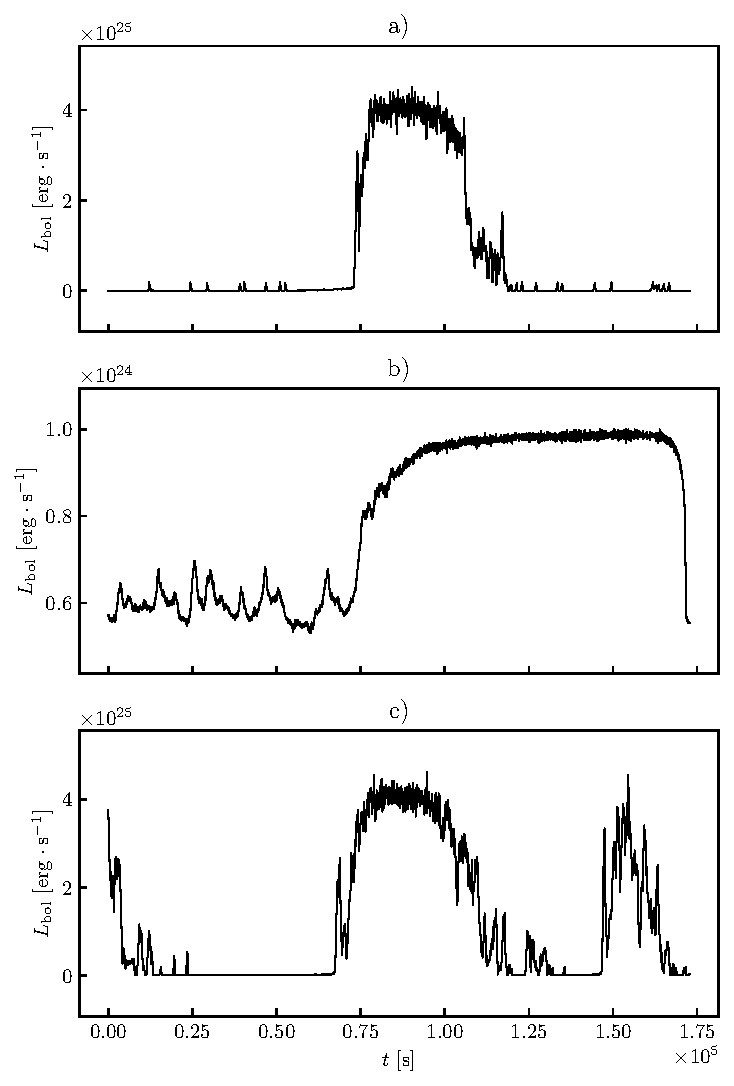
\includegraphics[width=1.0\textwidth]{img/plot_light_curves_disturbed.pdf}
    \end{center}
    \caption{Synthetic light curves extracted from the undisturbed SIM runs: \mbox{a) C5 ($q = 0.1$; $\psi = 0.9$), b) C6 ($q = 0.9$; $\psi = 0.1$), c) C7 ($q = 0.9$; $\psi = 0.9$)}}
    \label{fig:plot_light_curves_disturbed}
    \end{figure}

    % TODO: Radial flickering distribution plot

    
    % 9. ALPHA MODEL FITING
    %&<latex>
\chapter{$\alpha$-DISK MODEL FITTING}
\label{chap:alpha_model_fitting}
\thispagestyle{empty}
\mquote{I'm your density.}{George McFly}

In this relatively short Chapter, we use the results of undisturbed SIM runs presented in Chapter~\ref{chap:cv_models} to obtain the free parameter $\alpha$ of Shakura-Sunyaev's $\alpha$-disc model. To do that, we utilize the area density solution in the Shakura-Sunyaev solution set \eqref{eq:alpha_model_solution}, for which we will find the best $\alpha$ parameter fit for SIM cases C2, C3, and C5.

\section{Fitting the area density distribution}
    The Shakura-Sunyaev $\alpha$-disc solution for the area density profile is

    \begin{equation}
        \Sigma = 5.2 \alpha^{-4/5} \dot{M}^{7/10}_{16} m^{1/4}_1 R^{-3/4}_{10} f^{14/5}\ \si{\gram\ \cm^{-2}},
        \label{eq:density_analytical}
    \end{equation}

    where we will threat the $\dot{M}_{16}$ and $m_1$ values as constats, and the boundary layer function $f$ will have the radius $R_*$ fixed to the value of inner radius of the disc $r_{\mathrm{in}}$

    \begin{align}
        \begin{split}
            \dot{M}_{16} &= 0.01, \\
            m_1 &= 0.63 M_{\odot}, \\
            f &= \left[ 1 - \left( \frac{r_{\mathrm{in}}}{R} \right)^{1/2} \right]^{1/4}. \\
        \end{split}
    \end{align}

    Therefore, the only remaining variable to optimize the function \eqref{eq:density_analytical} for (i.e., the response variable) is the parameter $\alpha$, while the independent variable (i.e., the predictor) is the radius $R_{10}$. Figure~\ref{fig:plot_density_analytical} shows several examples of dependencies for equation~\eqref{eq:density_analytical} using different values of $\alpha$ parameter.  
    
    The density data used for fitting we get from the SIM runs C2, C4, and C5 by transforming the individual cell masses into densities with the use of the known surface area of the disc's cells. The second step is to calculate the mean area density $\bar{\Sigma}(R_{10})$ by averaging the cell's densities ring-wise and also over several hundred simulation steps ($200$ steps, in this case, to be precise). 

    \begin{figure}[H]
    \begin{center}
        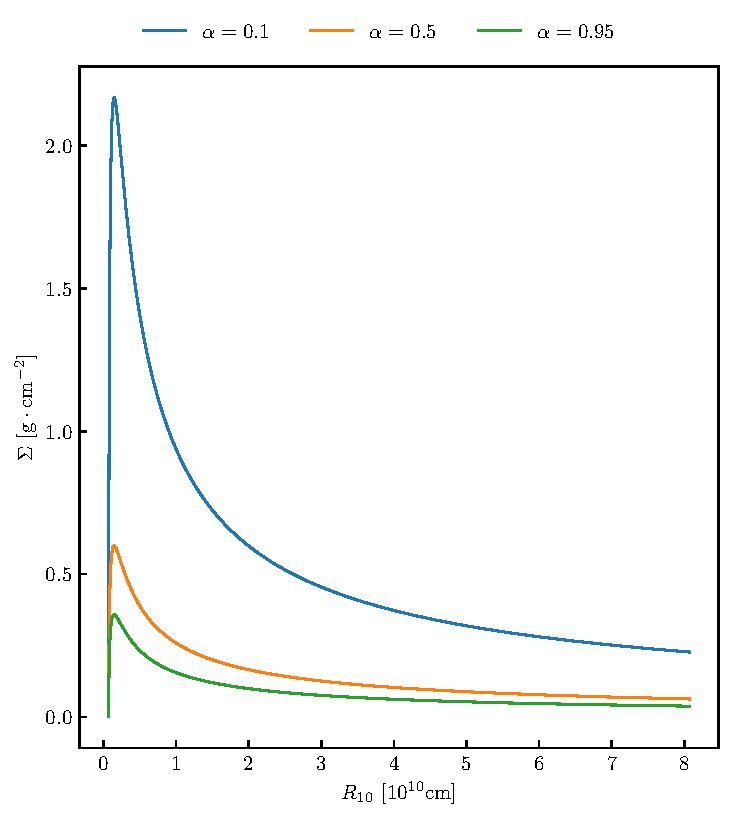
\includegraphics[width=1.0\textwidth]{img/plot_density_analytical.pdf}
    \end{center}
    \caption{Examples of Shakura-Sunyaev analytical area density solution.}
    \label{fig:plot_density_analytical}
    \end{figure}

    Figure~\ref{fig:plot_mean_density_fit} shows the Shakura-Sunyaev $\alpha$-disc area density $\Sigma$ solution~\eqref{eq:density_analytical} fited to mean area density data $\bar{\Sigma}$ extracted from C2, C3, and C4 SIM runs, respectivelly. The edge data (i.e., the inner and outer edge of the disc) were omitted from the fit because the irregular local conditions squee these data points. The outer edge's temperature and mass content are mostly a product of steady mass influx from the secondary component. To ensure numerical stability, the inner edge often triggers the low-value mass cut-off (see equation~\eqref{eq:m_cut_off}). 

    We can see that the MSH model produces a distribution that closely agrees with the analytical $\alpha$-disc solution. Therefore we can reliably obtain the value of the $\alpha$ parameter for specific MDH configurations. The particular value of $\alpha$ alpha could then be used to compute the distribution of other variables in the Shakura-Sunyaev solution set (see. equations~\eqref{eq:alpha_model_solution}).  
    
    \begin{figure}[H]
    \begin{center}
    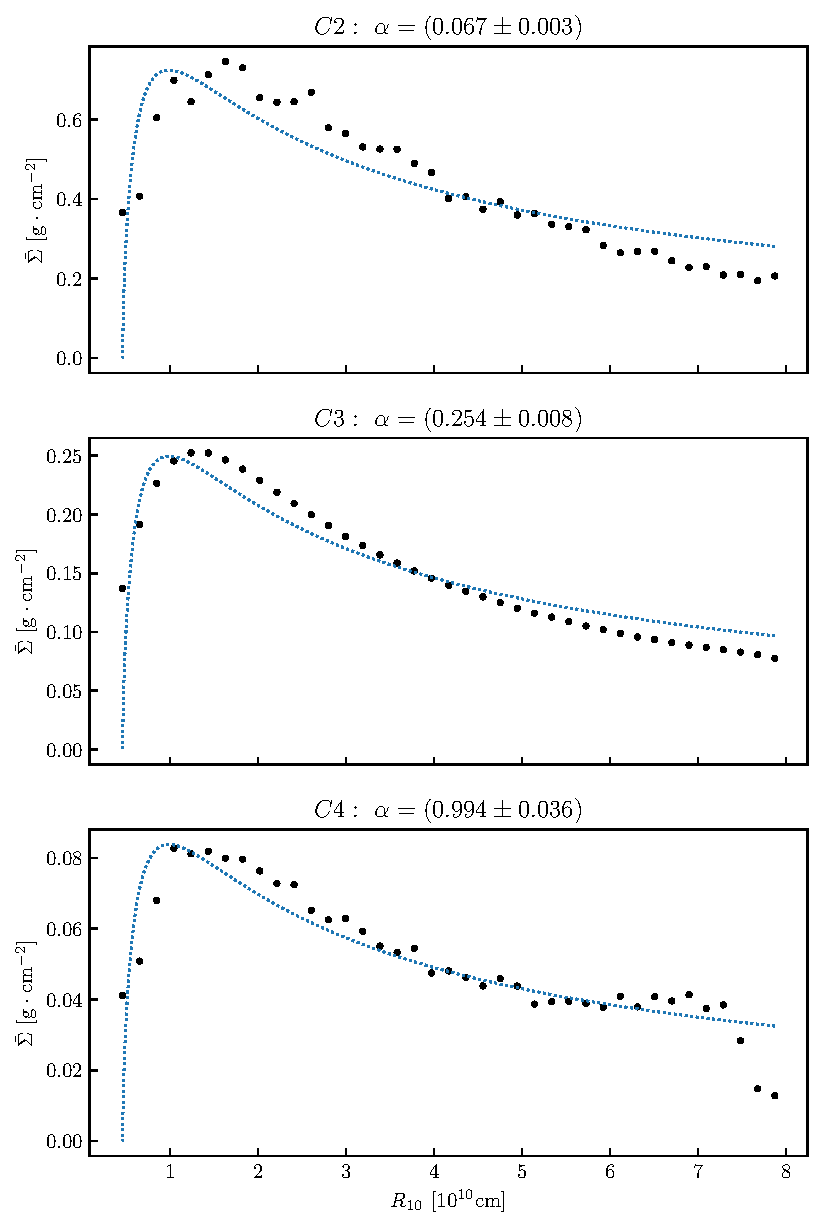
\includegraphics{img/plot_mean_density_fit.pdf}
    \end{center}
        \caption{Shakura-Sunyaev $\alpha$-parameter fits (dotted blue curves) for mean area density $\bar{\Sigma}$ extracted from C2 ($q=0.1, \psi=0.9$), C3 ($q=0.9, \psi=0.1$), and C4 ($q=0.9, \psi=0.9$) SIM runs. }
    \label{fig:plot_mean_density_fit}
    \end{figure}


    % DISCUSSION
    \chapter{DISCUSSION}
\thispagestyle{empty}
\mquote{...}{...}

% TODO: napsat kapitolu
% TODO: citát! 

    Over the course of this publication we provided a detailed description of our \emph{Multilayer accretion disc} (MDH) model (see Chapter~\ref{chap:multilayer_dripping_handrail}), did an overview of its specific code implementation (see Chapter~\ref{chap:model_implementation}), nad demostrated its capabilities on chosen generic CV system using several model configurations (see Chapter~\ref{chap:cv_models}). We then used these results to obtain specific values of Shakura-Sunyaev $\alpha$ parameter for each configuration. 

    In this last Chapter, we would like to disscuss the successes, limitations or failures regarding the specific topics of our research journey with the MDH model. Also we want to provide some questions, ideas or inspirations for our future research or the related research of others.
    
\section{MDH implementation}

\section{Simulations results}

\section{Determining the Shakura-Sunyaev $\alpha$ parameter}

\section{Future research questions and inspiration}



    \pagestyle{plain}

    % Seznam použitých zkratek
    \newpage
\phantomsection
\addcontentsline{toc}{chapter}{LIST OF ABBREVIATIONS}
\noindent \Large \textbf{LIST OF ABBREVIATIONS}
\normalsize

\vspace{1cm}

\begin{center}
\def\arraystretch{1.5}%
\setlength\tabcolsep{1cm}
\begin{tabular}{ll}
    CV			& cataclysmic variable star \\
    WD			& white dwarf star \\
    NS          & neutron star \\
    BH          & black hole \\
    YSO         & young stelar object \\
    AGN         & active galactic nuclei \\
    XB          & X-ray binary \\
    HMXB        & high-mass X-ray binary \\
    LMXB        & low-mass X-ray binary \\
    FDM			& fluid dynamical model \\
    MSM			& mass-spring model \\
    MSMM		& mass-spring model modified \\
    CA			& cellular automaton \\
    ODE			& ordinary differential equation
\end{tabular}
\end{center}


    % Seznam použitých konstant
    \newpage

\phantomsection
\addcontentsline{toc}{chapter}{LIST OF CONSTANTS}
\noindent \Large \textbf{LIST OF CONSTANTS}
\normalsize

\vspace{10mm}
\begin{center}

\begingroup
\def\arraystretch{1.5}

\begin{tabularx}{\textwidth}{ccX}
\hline
\hline
\textbf{Symbol}	& \textbf{Value [units]} & \textbf{Meaning} \\
\hline
\hline
$G$	&
	\begin{tabular}{c}
        $6.67430 \cdot 10^{-11}\ [\si{\newton \cdot \meter^2 \cdot \kilogram^{-2}}]$ \\
         $6.67430 \cdot 10^{-8}\ [\si{\mathrm{dyne} \cdot \cm^2 \cdot \gram^{-1}}]$
	\end{tabular} 
	& Gravitational const. \\

$h$ &
	\begin{tabular}{c}
        $6.6260755 \cdot 10^{-34}\ [\si{\meter^2 \cdot \kilogram \cdot \second^{-1}}] $ \\
         $6.6260755 \cdot 10^{-27}\ [\si{\cm^2 \cdot \gram \cdot \second^{-1}}]$
	\end{tabular} 
	& Planck's const. \\
	
$k$ &
	\begin{tabular}{c}
        $1.380658 \cdot 10^{-23}\ [\si{\meter^2 \cdot \kilogram \cdot \second^{-2} \cdot \kelvin^{-1}}]$ \\
        $1.380658 \cdot 10^{-16}\ [\si{\mathrm{erg} \cdot \kelvin^{-1}}]$
	\end{tabular} 
	& Boltzmann's const. \\
	
$\sigma$ &
	\begin{tabular}{c}
        $5.670374 \cdot 10^{-8}\ [\si{\watt \cdot \meter^{-2} \cdot \kelvin^{-4}}] $ \\
        $5.670374 \cdot 10^{-5}\ [\si{\mathrm{erg} \cdot \cm^{-2} \cdot \gram^{-1} \cdot \second^{-2}}]$
	\end{tabular} 
	& Stefan-Boltzmann's const. \\

$c$ &
	\begin{tabular}{c}
        $2.99792458 \cdot 10^{8}\ [\si{\meter \cdot \second^{-1}}]$ \\
         $2.99792458 \cdot 10^{10}\ [\si{\cm \cdot \second^{-1}}]$
	\end{tabular} 
	& Speed of light \\
	
$M_{\odot}$	&
	\begin{tabular}{c}
        $1.98847\cdot 10^{30}\ [\si{\kilogram}]$ \\
         $1.98847\cdot 10^{33}\ [\si{\gram}]$
	\end{tabular} 
	& Solar mass \\

$R_{\odot}$	&
	\begin{tabular}{c}
        $6.957\cdot 10^{8}\ [\si{\m}]$ \\
        $6.957\cdot 10^{10}\ [\si{\cm}]$
	\end{tabular} 
	& Solar radius \\
	
\hline

\end{tabularx}

\endgroup

\end{center}


    % Sezman figures/grafu
    % \newpage

\phantomsection
\addcontentsline{toc}{chapter}{LIST OF FIGURES}
\noindent \Large \textbf{LIST OF FIGURES}
\normalsize


    % Seznam literatury
    \newpage
\phantomsection
\addcontentsline{toc}{chapter}{REFERENCES}
\noindent \Large \textbf{REFERENCES}
\printbibliography[type=article,title={Articles},heading=subbibliography]
\printbibliography[type=book,title={Books},heading=subbibliography]
\printbibliography[type=thesis,title={Thesis},heading=subbibliography]
\printbibliography[type=misc,title={Miscellaneous},heading=subbibliography]

\end{document}
